%%%%%%%%%%%%%%%%%%%%%%%%%%%%%%%%%%%%%%%%%%%%%%%%%%%%%%%%%%%%%%%%%%%%%%%%%%%%%%%
% Author:  Pablo Alvarado
%
% Escuela de Ingeniería Electrónica
% Instituto Tecnológico de Costa Rica
%
% Tesis de Licenciatura
% 
% Phone:   +506 2550 9005
% email:   palvarado@itcr.ac.cr
%
%%%%%%%%%%%%%%%%%%%%%%%%%%%%%%%%%%%%%%%%%%%%%%%%%%%%%%%%%%%%%%%%%%%%%%%%%%%%%%%

% \documentclass is book
% If you want a printable two-side version of the thesis
%\documentclass[12pt,twoside,letterpaper]{book}

% If you want an electronic-only version of the thesis, do it one-sided
\documentclass[12pt,oneside,letterpaper]{book}

\usepackage[T1]{fontenc}
%\usepackage[utf8]{inputenc}   % is no longer required (since 2018)
\usepackage{ifthen}            % provide if-then-else operators

% --------------------------------------------------------------------------
% Global variables required in document formatting
% --------------------------------------------------------------------------
%
% BOOK MODE
%
\newboolean{bookmode}                  % boolean used to control book format
% Ensure that only one of the next two lines is active:
\setboolean{bookmode}{true}           % turn book mode on
%\setboolean{bookmode}{false}           % turn book mode off

%
% DRAFT MODE
%   The draft mode activates the TODO index and some "draft" markings all
%   around.  Ensure you set it to false for the final version!!
%   
%
\newboolean{draftmode}                  % boolean used to control draft-mode

%% -------------------------------------------------------------------------

%% Configure su nombre, título de tesis, lectores, fechas, etc. en:
%%
%% >>>>  config.tex  <<<<
%%

% --------------------------------------------------------------------------

% include all packages and define all required general macros
%%%%%%%%%%%%%%%%%%%%%%%%%%%%%%%%%%%%%%%%%%%%%%%%%%%%%%%%%%%%%%%%%%%%%%%%%%%%%%%
% Author:  Pablo Alvarado
%
% Escuela de Electrónica
% Instituto Tecnológico de Costa Rica
%
% Phone:   +506 2550 9005
% email:   palvarado@itcr.ac.cr
% 
%%%%%%%%%%%%%%%%%%%%%%%%%%%%%%%%%%%%%%%%%%%%%%%%%%%%%%%%%%%%%%%%%%%%%%%%%%%%%%%

\PassOptionsToPackage{usenames,dvipsnames}{xcolor}

% -----------------------------------------------------------------------------
%   Define all configuration commands
% -----------------------------------------------------------------------------

\newcommand{\genderLector}[1]{%
  \ifthenelse{\equal{#1}{F}}{%
    Profesora Lectora%
  }{%
    \ifthenelse{\equal{#1}{M}}{%
      Profesor Lector%
    }{%
      Persona profesora lectora%
    }%
  }%
}

% Lector I
\newcommand{\nameLectorI}{$<$\emph{Use defLectorI in config.tex}$>$}
\newcommand{\genderLectorI}{N/A}

\newcommand{\defLectorI}[1][M]{%
  \renewcommand{\genderLectorI}{\genderLector{#1}}%
  \lectorIRelay%
}

\newcommand{\lectorIRelay}[1]{%
  \renewcommand{\nameLectorI}{#1}
}

%% Lector II
\newcommand{\nameLectorII}{$<$\emph{Use setLectorII in main.tex}$>$}
\newcommand{\genderLectorII}{N/A}

\newcommand{\defLectorII}[1][M]{%
  \renewcommand{\genderLectorII}{\genderLector{#1}}%
  \lectorIIRelay%
}

\newcommand{\lectorIIRelay}[1]{%
  \renewcommand{\nameLectorII}{#1}
}

%% Asesor
\newcommand{\nameAsesor}{$<$\emph{Use setAsesor in main.tex}$>$}
\newcommand{\genderAsesor}{$<$\emph{Use setAsesor in main.tex}$>$}

\newcommand{\defAsesor}[1][M]{%
  \ifthenelse{\equal{#1}{F}}{%
    \renewcommand{\genderAsesor}{Profesora Asesora}%
  }{%
    \ifthenelse{\equal{#1}{M}}{%
      \renewcommand{\genderAsesor}{Profesor Asesor}%
    }{%
      % La RAE no ha definido cómo hacer esto...
      %
      % Hay que preguntar a la persona asesora no-binaria directamente
      % cómo gusta ser tratada.
      \renewcommand{\genderAsesor}{Persona profesora asesora}%
    }
  }
  \asesorRelay
}

\newcommand{\asesorRelay}[1]{%
  \renewcommand{\nameAsesor}{#1}
}

% Dates for draft and final
\newcommand{\thesisDraftDate}{\today}
\newcommand{\defDraftDate}[1]{\renewcommand{\thesisDraftDate}{#1}}

\newcommand{\thesisFinalDate}{$<$\emph{Fecha de Defensa en config.tex}$>$}
\newcommand{\defFinalDate}[1]{\renewcommand{\thesisFinalDate}{#1}}

% Author definition and gender related strings

\newcommand{\thesisAuthor}{Error: Undefined}
\newcommand{\thesisAuthorShort}{Error: Undefined}
\newcommand{\thesisAuthorTECID}{Error: Undefined}
\newcommand{\thesisAuthorAddress}{Error: Undefined}
\newcommand{\thesisAuthorDegree}{Error: Undefined}

\newcommand{\defAuthor}[1][M]{%
  \ifthenelse{\equal{#1}{F}}{%
    \renewcommand{\thesisAuthorAddress}{la señora}
    \renewcommand{\thesisAuthorDegree}{Ingeniera}
  }{%
    \ifthenelse{\equal{#1}{f}}{%
      \renewcommand{\thesisAuthorAddress}{la señorita}
      \renewcommand{\thesisAuthorDegree}{Ingeniera}
    }{%
      \ifthenelse{\equal{#1}{M}}{%
        \renewcommand{\thesisAuthorAddress}{el señor}
        \renewcommand{\thesisAuthorDegree}{Ingeniero}
        
      }{%
        \renewcommand{\thesisAuthorAddress}{la persona}
        \renewcommand{\thesisAuthorDegree}{Ingeniere}
      }
    }
  }
  \authorRelay
}

\newcommand{\authorRelay}[1]{%
  \renewcommand{\thesisAuthor}{#1}
}

\newcommand{\defAuthorShort}[1]{%
  \renewcommand{\thesisAuthorShort}{#1}
}

\newcommand{\defAuthorTECID}[1]{%
  \renewcommand{\thesisAuthorTECID}{#1}
}

%% About the institution and department
\newcommand{\thesisDepartment}{Escuela de Ingeniería Electrónica}
\newcommand{\thesisInstitution}{Tecnológico de Costa Rica}

\newcommand{\defDepartment}[1]{%
  \renewcommand{\thesisDepartment}{#1}
}

\newcommand{\defInstitution}[1]{%
  \renewcommand{\thesisInstitution}{#1}
}



%% About the report name, and type
\newcommand{\thesisTitle}{Error: Undefined}
\newcommand{\thesisFlatTitle}{\thesisTitle}
\newcommand{\thesisKeywords}{Error: Undefined}
\newcommand{\thesisType}{Error: Undefined}

%% A tool to remove new lines leaving no spaces
\newcommand\titleFlattener[1]{\def\\{\relax\ifhmode\unskip\fi\space\ignorespaces}#1}

\newcommand{\defTitle}[1]{%
  \renewcommand{\thesisFlatTitle}{\titleFlattener{#1}}
  \renewcommand{\thesisTitle}{#1}
}

\newcommand{\defKeywords}[1]{%
  \renewcommand{\thesisKeywords}{#1}
}

\newcommand{\defTFGType}[1]{%
  \renewcommand{\thesisType}{#1}
}

%% Este archivo contiene toda la configuración básica del documento de
%% tesis, para centralizar alguna información que se requiere en todo
%% el documento.

%% DRAFT MODE

%%   El modo borrador activa las listas de cosas por hacer, con su
%%   índice, y algunas marcas explícitas de "borrador" por todo lado.
%%
%%   Asegúrse de que esta variable sea false en la versión final y de haber
%%   actualizado la fecha de la defensa, un poco más abajo.
\setboolean{draftmode}{true}            % turn draft mode on
%\setboolean{draftmode}{false}          % turn draft mode off

%% Esta es la fecha que se colocará en el modo borrador
\defDraftDate{\today}
%% Esta es la fecha que se usará en la versión final
\defFinalDate{July 16, 2023}

%% Este es el nombre del estudiante y el pronombre que utiliza, para cambiar
%% las portadas como corresponde

% Con el nombre de autor, se debe especificar el género a utilizar:
%
%   [M]asculino
%   [F]emenino (usando "señora" donde corresponda)
%   [f]emenino (usando "señorita" donde corresponda)
%   persona [N]o binaria
%
%   Debido a la falta de norma en español para las personas no binarias,
%   posíblemente deba ajustarse para el gusto de cada quien.
%
\defAuthor[M]{Francis Guindon Badilla}                % Nombre del estudiante
%\defAuthor[f]{María del Pilar Pérez Prado}    % Nombre de la estudiante

\defAuthorShort{F.~Guindon}                      % Nombre corto
\defAuthorTECID{2018259419}                     % Carné

%% Este es el título completo del informe del trabajo final de graduación.
%% Usted puede agregar \\ para forzar líneas nuevas en la portada y automática-
%% mente el comando se encarga de eliminar eso cuando necesita el título
% \defTitle{Detección de artefactos de video \\%
% en tiempo real sobre un sistema embebido}
\defTitle{Embedded soft real time video artifact detector}

%% Palabras clave
\defKeywords{}

%% Tribunal Evaluador
%%
%% Indique los nombres de los lectores y asesor
%% El parámetro opcional es
%%  [M]asculino,
%%  [F]emenino,
%%  persona [N]o binaria
\defAsesor[M]{Dr.\,Pablo Alvarado}
\defLectorI[M]{Dr.\,Jorge Castro Godinez}
\defLectorII[M]{Dr.\,Pablo Mendoza Ponce}


%% Tipo de tesis o informe
%%   - Tesis de Licenciatura
%%   - Informe de Proyecto Final 
%%   - Tesis de Maestría
\defTFGType{Tesis de Licenciatura}

%% Nombre del departamento e institución
\defInstitution{Instituto Tecnológico de Costa Rica}
\defDepartment{Escuela de Ingeniería Electrónica}

 % Load the desired configuration

%Para el PDF (cambiar si se desea otras cosas a lo indicado arriba
\newcommand{\pdfAuthor}{\thesisAuthor}
\newcommand{\pdfTitle}{\thesisFlatTitle} 
\newcommand{\pdfKeywords}{\thesisKeywords}
\newcommand{\pdfSubject}{\thesisType}


%% -------------------------------------------------------------------

\usepackage{ifpdf}

% Command to change between draft or release mode:
\newcommand{\ifdraft}[2]{\ifthenelse{\boolean{draftmode}}{#1}{#2}}
% Command to change between draft or release mode:
\newcommand{\ifbook}[2]{\ifthenelse{\boolean{bookmode}}{#1}{#2}}

% include all required packages here
\usepackage{csquotes}                  % recommended for biblatex
\usepackage[spanish,es-tabla]{babel}   % spanish, remove es-tabla for cuadro
%\usepackage[spanish]{babel}   % spanish, remove es-tabla for cuadro

\usepackage{xspace} % Decide if a space is needed at the end of some commands

\makeatletter
% babel uses a hook and therefore the tablename is here not defined yet.
% However, it defines es@tablename with upper/lowercase, and we use it.
\ifthenelse{\equal{\es@tablename}{Ttabla}}{%
  \newcommand{\cuadro}{tabla}
  \newcommand{\cuadros}{tablas}
  \newcommand{\Cuadro}{Tabla}
  \newcommand{\elcuadro}{la tabla}
  \newcommand{\Elcuadro}{La tabla}
  \newcommand{\loscuadros}{las tablas}
  \newcommand{\Loscuadros}{Las tablas}
  
  \newcommand{\tabla}{tabla}
  \newcommand{\tablas}{tablas}
  \newcommand{\Tabla}{Tabla}
  \newcommand{\latabla}{la tabla}
  \newcommand{\Latabla}{La tabla}
  \newcommand{\lastablas}{las tablas}
  \newcommand{\Lastablas}{Las tablas}
  
  \newcommand{\tabref}[1]{\hyperref[#1]{tabla~\ref*{#1}}\xspace}
  \newcommand{\Tabref}[1]{\hyperref[#1]{Tabla~\ref*{#1}}\xspace}

  \newcommand{\latabref}[1]{la \tabref{#1}}
  \newcommand{\Latabref}[1]{La \tabref{#1}}

}{%
  \newcommand{\cuadro}{cuadro}
  \newcommand{\cuadros}{cuadros}
  \newcommand{\Cuadro}{Cuadro}
  \newcommand{\elcuadro}{el cuadro}
  \newcommand{\Elcuadro}{El cuadro}
  \newcommand{\loscuadros}{los cuadros}
  \newcommand{\Loscuadros}{Los cuadros}
  
  \newcommand{\tabla}{cuadro}
  \newcommand{\tablas}{cuadros}
  \newcommand{\Tabla}{Cuadro}
  \newcommand{\latabla}{el cuadro}
  \newcommand{\Latabla}{El cuadro}
  \newcommand{\lastablas}{los cuadros}
  \newcommand{\Lastablas}{Los cuadros}
  
  \newcommand{\tabref}[1]{\hyperref[#1]{cuadro~\ref*{#1}}\xspace}
  \newcommand{\Tabref}[1]{\hyperref[#1]{Cuadro~\ref*{#1}}\xspace}

  \newcommand{\latabref}[1]{el \tabref{#1}}
  \newcommand{\Latabref}[1]{El \tabref{#1}}

}
\makeatother

% References to figures
\newcommand{\figref}[1]{\hyperref[#1]{figura~\ref*{#1}}\xspace}
\newcommand{\Figref}[1]{\hyperref[#1]{Figura~\ref*{#1}}\xspace}
\newcommand{\lafigref}[1]{la \hyperref[#1]{figura~\ref*{#1}}\xspace}
\newcommand{\Lafigref}[1]{La \hyperref[#1]{figura~\ref*{#1}}\xspace}

% References to equations
\newcommand{\equ}[1]{\hyperref[#1]{(\ref*{#1})}\xspace}

% Refrences to chapters and sections
\newcommand{\capref}[1]{\hyperref[#1]{capítulo~\ref{#1}}\xspace}
\newcommand{\secref}[1]{\hyperref[#1]{sección~\ref{#1}}\xspace}

\usepackage{makeidx}                    % to create index file

\usepackage[nottoc]{tocbibind}          % Fix the hyperrefs to TOC,TOF, etc.
                                        % and ensure that they appear all in 
                                        % the Table of Contents
\ifdraft{%
  %\usepackage[refpage]{nomencl}        % Use to easily administrate the list
  \usepackage[intoc,spanish]{nomencl}   % of symbols
}{%
  \usepackage[intoc,spanish]{nomencl}
}

\usepackage{siunitx}                    % Units of the SI
\sisetup{output-decimal-marker = {,}}   % Use decimal , instead of decimal .
\DeclareSIQualifier\peak{p}
\DeclareSIQualifier\ppeak{pp}

\usepackage{amsmath}
\usepackage{amssymb,amstext}            % AMS-math and symbols package
\usepackage{mathrsfs}                   % Calygraphic fonts for transforms
\usepackage{trsym}                      % Para símbolos de transformadas o---o
\usepackage{stmaryrd}                   % For short arrows
\usepackage{nicefrac}
\usepackage{array}                      % extensions to tabular environment
\usepackage{longtable}                  % supports extraordinary long tables
\usepackage{tabularx}                   % supports tables with fixed width

\usepackage[backend=biber,              % Use biber/biblatex
            style=ieee,
            sorting=none,
            citestyle=numeric-comp]{biblatex}

\usepackage{afterpage}                  % put something only after the page
\usepackage{multirow}                   % supports multiple row grouping in 
                                        % tables
\usepackage{multicol}                   % multiple columns environments
\usepackage{enumitem}                   % better enumeration with paralist 
                                        % equivalents as follows:

\newlist{compactitem}{itemize}{3}
\setlist[compactitem]{topsep=0pt,partopsep=0pt,itemsep=0pt,parsep=0pt}
\setlist[compactitem,1]{label=\textbullet}
\setlist[compactitem,2]{label=---}
\setlist[compactitem,3]{label=*}

\newlist{compactdesc}{description}{3}
\setlist[compactdesc]{topsep=0pt,partopsep=0pt,itemsep=0pt,parsep=0pt}

\newlist{compactenum}{enumerate}{3}
\setlist[compactenum]{label*=\arabic*.,topsep=0pt,partopsep=0pt,itemsep=0pt,parsep=0pt}
\newlist{compactenuma}{enumerate}{3}
\setlist[compactenuma]{label*=\alph*.,topsep=0pt,partopsep=0pt,itemsep=0pt,parsep=0pt}

\usepackage{icomma}                     % decimal comma in math mode

\usepackage{bold-extra}

\usepackage[format=hang,%
            font=small,%
            labelfont=bf]{caption}      % nicer figure captions
\usepackage{subcaption}                 % for subfigures
            
\usepackage{booktabs}                   % book type tabulars
\usepackage{pdfpages}                   % used to include the final "acta"

% the own style with options depending on the draft mode
\ifdraft{%
\usepackage[todo]{sty/tecStyle}         % some command definitions
                                        % options [todo] todo-index
}{%
\usepackage{sty/tecStyle}               % some command definitions
                                        % options [todo] todo-index
}

%% fix the title for examples
\renewcommand{\examplelistname}{Índice de ejemplos}
\renewcommand{\examplename}{Ejemplo}

%% define some command to cope with the tribunal names

%% Lector I


\usepackage{url}                        % allows linebreaks at certain
                                        % characters or combinations of 
                                        % characters for URLs

%% Usual tikz libraries and configuration
\usepackage{tikz}
\usepackage{pgfplots}
\pgfplotsset{compat=1.16}
\usepgfplotslibrary{fillbetween}
\usetikzlibrary{patterns,shapes,arrows.meta,positioning,calc,babel}
\usetikzlibrary{fit,shapes.geometric,decorations.markings}

\usepackage{listings}                   % syntax highlighting of code fragments

\lstdefinestyle{verilog-style}
{
  language=Verilog,
  basicstyle=\small\ttfamily,
  keywordstyle=\color{dkblue},
  identifierstyle=\color{black},
  commentstyle=\color{dkgreen},
  numbers=left,
  numberstyle=\tiny\color{black},
  numbersep=10pt,
  tabsize=8,
  moredelim=*[s][\colorIndex]{[}{]},
  literate=*{:}{:}1
}
\lstset{literate=%
  {á}{{\'a}}1
  {é}{{\'e}}1
  {í}{{\'i}}1
  {ó}{{\'o}}1
  {ú}{{\'u}}1
  {ñ}{{\~n}}1
  {Á}{{\'A}}1
  {É}{{\'E}}1
  {Í}{{\'I}}1
  {Ó}{{\'O}}1
  {Ú}{{\'U}}1
  {Ñ}{{\~N}}1
}

\definecolor{vorange}{RGB}{255,143,102}

\makeatletter
\newcommand*\@lbracket{[}
\newcommand*\@rbracket{]}
\newcommand*\@colon{:}
\newcommand*\colorIndex{%
    \edef\@temp{\the\lst@token}%
    \ifx\@temp\@lbracket \color{black}%
    \else\ifx\@temp\@rbracket \color{black}%
    \else\ifx\@temp\@colon \color{black}%
    \else \color{vorange}%
    \fi\fi\fi
}
\makeatother


% For pdflatex
% - The hyperref package should always be loaded last, since it has to
%   overwrite some of the commands.
% - The package subfigure caused that the pagebackrefs and index refs were set
%   incorrectly.

\ifpdf
%
% final / draft document options
%\usepackage{graphicx}                   % for inserting pdf-graphics.
                                        % options final / draft
\ifdraft{%
\usepackage[%pdftex,%
            naturalnames=true,
            linktocpage,
            hyperindex,
            colorlinks,
            urlcolor=dkred,          %\href to external url
            filecolor=dkmagenta,     %\href to local file
            linkcolor=dkred,         %\ref and \pageref
            citecolor=dkgreen,       %\cite
            plainpages=false,
            pdfpagelabels,
            pdfpagemode=UseOutlines, % means use bookmarks (None,UseOutlines)
            % bookmarksopen=false,   % would show the whole hierarchy if true
            bookmarksnumbered=true,
            pdfpagelayout=OneColumn, % SinglePage,OneColumn,TwoColumnLeft,...
            pdfview=FitH, % FitB,FitBH,FitBV,Fit,FitH,FitV
            pdfstartview=FitH, % FitB,FitBH,FitBV,Fit,FitH,FitV
            unicode,
            ]{hyperref}
}{%
% Use biber/biblatex
\usepackage[%pdftex,%
            naturalnames=true,
            linktocpage,hyperindex,
            colorlinks,
            urlcolor=dkred,          %\href to external url
            filecolor=dkmagenta,     %\href to local file
            linkcolor=dkred,         %\ref and \pageref
            citecolor=dkgreen,       %\cite
            plainpages=false,
            pdfpagelabels,
            pdfpagemode=UseOutlines, % means use bookmarks (None,UseOutlines)
            % bookmarksopen=false,   % open the whole hierarchy if true!
            bookmarksnumbered=true,
            pdfpagelayout=OneColumn, % SinglePage,OneColumn,TwoColumnLeft,...
            pdfview=FitH, % FitB,FitBH,FitBV,Fit,FitH,FitV
            pdfstartview=FitH, % FitB,FitBH,FitBV,Fit,FitH,FitV,
            unicode,
            ]{hyperref}
}


%
% Ensure that the links of the images point to the top of the images and not
% to the caption
%
\usepackage[figure]{hypcap}

% %
% % Ensure that pdfLaTeX do the same spacing as LaTeX
% %
\pdfadjustspacing=1 
% %
\else   % i.e. if not pdf

\usepackage[active]{srcltx}             % insert links into the dvi to jump
\usepackage{graphicx}                   % for inserting eps-graphics.
                                        % options final / draft
                                        % into the sources directly.
\ifdraft{%
\usepackage[ps2pdf,%
            % plainpages=false,
            linktocpage,
            hyperindex,
            % pdfpagelabels,
            pdfpagemode=UseOutlines,
            pdfstartview=FitH,
            unicode,]{hyperref}
}{%
\usepackage[ps2pdf,%
            % plainpages=false,
            linktocpage,
            hyperindex,
            % pdfpagelabels,
            pdfpagemode=UseOutlines,
            pdfstartview=FitH,
            unicode,]{hyperref}
}

%\usepackage[ps2pdf]{hyperref}

\fi  % end of if pdf or not

% --------------------------------------------------------------------------

% Allow the use of international characters
\AtBeginDocument{%
  \hypersetup{%
             pdftitle={\pdfTitle},%
             pdfsubject={\pdfSubject},%
             pdfauthor={\pdfAuthor},%
             pdfkeywords={\pdfKeywords}
            }%
}


%\usepackage{algorithmic}            % algorithmic environment


\usepackage{rotating}                % allow block rotation

%% This environment will allow to rotate a page in the PDF, just
%% for visualization purposes.  Since nowadays the documents are
%% almost never printed, it is best if rotated pages are also shown
%% rotated in the PDF viewer, and this is the purpose of this environment.
\newenvironment{rotatepage}%
{\global\pdfpageattr\expandafter{\the\pdfpageattr/Rotate 90}}%
{\clearpage\pagebreak[4]\global\pdfpageattr\expandafter{\the\pdfpageattr/Rotate 0}}

    
%%%%%%%%%%%%%%%%%%%%%%%%%%%%%%%%%%%%%%%%%%%%%%%%%%%%%%%%%%%%%%%%%%%%%%%%%%%%%%%

%\sloppy

%
% Some own font definitions
%
\DeclareMathAlphabet{\mathpzc}{OT1}{pzc}{m}{it}
\DeclareMathAlphabet{\mathpss}{OT1}{cmss}{m}{sl}

%
% page layout
%

\usepackage{vmargin}
\setpapersize{USletter}

% For letter-paper printing
\setmarginsrb{33mm}{8mm}{23mm}{7mm}{15pt}{15pt}{7mm}{12mm}
%\setlength{\headheight}{15pt}         % fancy headers wanted this

%
% Fraction of Float Object / Text
%

\renewcommand{\topfraction}{0.95}       % how much of top of page should be 
                                        % allowed to be float object?
\renewcommand{\bottomfraction}{0.95}    % how much of bottom of page should be
                                        % allowed to be float object?
\renewcommand{\textfraction}{0.05}      % how much of page must be text?

\usepackage{fancyhdr}                   % fancy page headers

\usepackage{lastpage}

%
% header and footer layout (needs package fancyhdr)
%
\newcommand{\copyrightfooter}{\tiny{\copyright \the\year\ --- \thesisAuthorShort %
    \qquad Uso exclusivo ITCR}}
%
\newcommand{\draftfoot}%
  {\ifdraft{\textcolor{dkblue}{\tiny\textsl{Borrador: \today}}{}}
           {}
}

\pagestyle{fancy}
\renewcommand{\chaptermark}[1]{\markboth{{\small
    \thechapter\hspace*{1mm}#1}}{}}
\renewcommand{\sectionmark}[1]{\markright{{\small
    \thesection\hspace*{1mm}#1}}{}}
%\lhead[{\small\textsc\Roman{\thepage}}]{\fancyplain{}%
\lhead[{\small\thepage}]{\fancyplain{}%
        {{\slshape \small\nouppercase{\leftmark}}}}
\chead[]{}
\rhead[\fancyplain{}%
%        {{\slshape \small\nouppercase{\rightmark}}}]{{\small\textsc\Roman{\thepage}}}
        {{\slshape \small\nouppercase{\rightmark}}}]{{\small\thepage}}
\lfoot[]{\draftfoot}
\ifbook{%
  \cfoot[]{}
}{
  \cfoot[\copyrightfooter]{\copyrightfooter}
}
\rfoot[\draftfoot]{}
\renewcommand{\headrulewidth}{0.5pt}
\renewcommand{\footrulewidth}{0pt}

%
% Caption style for tables
% For caption v3:
\captionsetup[table]{position=top,
  format=hang,
  textfont={normalsize},
  labelfont={normalsize,bf}}

\newcommand{\tablecaption}[2][foo]{%
  \ifthenelse{\equal{#1}{foo}}{%
    \caption{#2}%
  }{%
    \caption[#1]{#2}%
  }
}

%% En español hay diferencia entre Tabla y Cuadro.
%%
%% Tabla: es la tabla periódica, o una tabla de logaritmos o de
%%        probabilidades o de integrales. Usualmente es algo que no
%%        requiere referencias o explicaciones adicionales en el texto porque
%%        todas sus entradas son sucesiones de alguna cosa que se busca allí
%%        mismo
%% Cuadro: es lo que usualmente se usa en inglés como "table", y resume
%%        información que requiere al menos parcialmente explicaciones en el
%%        el texto.

%% \addto\extrasspanish{\renewcommand{\tablename}{Tabla}}
%% \addto\extrasspanish{\renewcommand{\listtablename}{\'Indice de tablas}}

%
% paragraph layout
%
\renewcommand{\baselinestretch}{1.1}    % line spacing
\parindent0em                           % indentation width of first line
\parskip1.3ex                           % space between paragraphs

%
% document consists of
% chapter - section - subsection - subsubsection - paragraph - subparagraph
%
\setcounter{secnumdepth}{2}             % depth of section numbering
\setcounter{tocdepth}{2}                % depth of table of contents

% For biblatex
\addbibresource{literatura.bib}

%
% prepares index from entries like \index{word} or \index{group!word}.
% don't forget to call "makeindex filename" for final index generation.
%
\makeindex                            %% for package makeidx.sty
%\newindex{default}{idx}{ind}{Index}  %% for package index.sty

\newcommand{\octave}{GNU/Octave}
\newcommand{\linux}{GNU/Linux}


%
% prepares notation or nomenclature 
%
\makenomenclature

%%% Local Variables: 
%%% mode: latex
%%% TeX-master: "main"
%%% End: 


% define all symbols used in the document
%% ---------------------------------------------------------------------------
%% paNotation.tex
%%
%% Notation
%%
%% $Id: notation.tex 1467 2010-07-24 16:47:17Z palvarado $
%% ---------------------------------------------------------------------------

\newcommand{\nms}{\negmedspace}

%%
% Command definitions for localized symbol format definition
%%
\renewcommand{\Re}{\operatorname{Re}}
\renewcommand{\Im}{\operatorname{Im}}

\newcommand{\prt}[1]{\ensuremath{\mathcal{#1}}}         %% partitioning
\newcommand{\img}[1]{\ensuremath{\mathcal{#1}}}         %% image as a set
\newcommand{\reg}[1][R]{\ensuremath{\mathcal{#1}}}      %% region
\newcommand{\pred}[1]{\ensuremath{\mathrm{#1}}}         %% predicate
\newcommand{\operat}[2]{\mathcal{#1}\left\{#2\right\}}
\newcommand{\transf}[1]{\mathscr{#1}}
\newcommand{\fourier}[1]{\transf{F}\left\{#1\right\}}
\newcommand{\ifourier}[1]{\transf{F}^{-1}\left\{#1\right\}}
\newcommand{\laplace}[1]{\transf{L}\left\{#1\right\}}
\newcommand{\ulaplace}[1]{\transf{L}_u\left\{#1\right\}}
\newcommand{\blaplace}[1]{\transf{L}_b\left\{#1\right\}}
\newcommand{\ilaplace}[1]{\transf{L}^{-1}\left\{#1\right\}}
\newcommand{\ztrans}[1]{\transf{Z}\left\{#1\right\}}
\newcommand{\iztrans}[1]{\transf{Z}^{-1}\left\{#1\right\}}
\newcommand{\zutrans}[1]{\transf{Z}_u\left\{#1\right\}}
\newcommand{\exceq}{\ensuremath{\overset{!}{=}}}

\newcommand{\signum}{\operatorname{signum}}
\newcommand{\vct}[1]{\ensuremath{\underline{\mathbf{#1}}}}
\newcommand{\mat}[1]{\ensuremath{\mathbf{#1}}}
\newcommand{\vctmu}{\vct{\boldsymbol{\mu}}}
\newcommand{\vctzeta}{\vct{\boldsymbol{\zeta}}}
\newcommand{\vctpi}{\vct{\boldsymbol{\pi}}}
\newcommand{\vctvarphi}{\vct{\boldsymbol{\varphi}}}
\newcommand{\raum}[1]{\ensuremath{\mathbb{#1}}}
\newcommand{\matSigma}{\mat{\boldsymbol{\Sigma}}}
\newcommand{\matLambda}{\mat{\boldsymbol{\Lambda}}}
\newcommand{\matPsi}{\mat{\boldsymbol{\Psi}}}
\newcommand{\matPhi}{\mat{\boldsymbol{\Phi}}}
\newcommand{\row}[2]{\ensuremath{\mathbf{\underline{#1}_{#2(\cdot)}}}}
\newcommand{\col}[2]{\ensuremath{\mathbf{\underline{#1}_{(\cdot) #2}}}}
\newcommand{\seq}[1]{\ensuremath{#1}}
\newcommand{\set}[1]{\ensuremath{\mathcal{#1}}}
\newcommand{\gset}[1]{\ensuremath{#1}} %% set for greek symbols
\newcommand{\front}[1]{\widehat{\set{#1}}}
\newcommand{\setlambda}{\set{\boldsymbol{\lambda}}}
\newcommand{\klass}[1]{\ensuremath{\mathpss{#1}}}
\newcommand{\graph}[1]{\ensuremath{\mathsf{#1}}}
\newcommand{\lab}[1]{\ensuremath{\mathpss{L}(#1)}}
\newcommand{\myfrac}[2]{{\footnotesize #1/#2}}
\newcommand{\ifthenspc}{\rule{3mm}{0mm}}
\newcommand{\point}[1]{\ensuremath{\mathsf{#1}}}
\newcommand{\estim}[1]{\ensuremath{\hat{#1}}}
\newcommand{\numset}[1]{\ensuremath{\mathbb{#1}}}
\newcommand{\tuple}[1]{\ensuremath{\left\langle#1\right\rangle}}
\newcommand{\norm}[1]{\ensuremath{\left\lVert#1\right\rVert}}
\newcommand{\conj}[1]{\ensuremath{{{#1}^{\ast}}}}
\newcommand{\base}[1]{\set{#1}}
\newcommand{\zeron}[1]{\ensuremath{\underset{\uparrow}{#1}}}
\newcommand{\sysT}{\ensuremath{\mathcal{T}}}
\newcommand{\sys}[1]{\ensuremath{\sysT\left[#1\right]}}
%\newcommand{\sen}{\operatorname{sen}} % sinus in spanish (seno)
%\newcommand{\senh}{\operatorname{senh}} % sinus hiperbolicus in spanish (seno)
%\newcommand{\arcsen}{\operatorname{arcsen}} % arcus sinus hiperbolicus in spanish (arcoseno)
\newcommand{\sgn}{\operatorname{sgn}} % signus
\newcommand{\roc}{\text{ROC: }}

\newcommand{\code}[1]{\texttt{#1}}
\newcommand{\conv}{\ensuremath{\ast}}
\newcommand{\cconv}{\ensuremath{\;\,\text{\footnotesize{N}}\!\!\!\!\!\!\bigcirc}}
\newcommand{\Ln}{\operatorname{Ln}}
\newcommand{\rand}{\operatorname{rand}}
\newcommand{\sa}{\operatorname{sa}}
\newcommand{\senc}{\operatorname{senc}}


%% Natural, Integer and Real Numbers
\newcommand{\setA}{\ensuremath{\mathbb{A}}}
\newcommand{\setB}{\ensuremath{\mathrm{I\negthinspace B}}}
\newcommand{\setC}{\ensuremath{\mathbb{C}}}
\newcommand{\setD}{\ensuremath{\mathrm{I\negthinspace D}}}
\newcommand{\setE}{\ensuremath{\mathrm{I\negthinspace E}}}
\newcommand{\setF}{\ensuremath{\mathrm{I\negthinspace F}}}
\newcommand{\setG}{\ensuremath{\mathbb{G}}}
\newcommand{\setH}{\ensuremath{\mathrm{I\negthinspace H}}}
\newcommand{\setI}{\ensuremath{\mathbb{I}}}
\newcommand{\setJ}{\ensuremath{\mathbb{J}}}
\newcommand{\setK}{\ensuremath{\mathrm{I\negthinspace K}}}
\newcommand{\setL}{\ensuremath{\mathrm{I\negthinspace L}}}
\newcommand{\setM}{\ensuremath{\mathrm{I\negthinspace M}}}
\newcommand{\setN}{\ensuremath{\mathrm{I\negthinspace N}}}
\newcommand{\setO}{\ensuremath{\mathbb{O}}}
\newcommand{\setP}{\ensuremath{\mathrm{I\negthinspace P}}}
\newcommand{\setQ}{\ensuremath{\mathbb{Q}}}
\newcommand{\setR}{\ensuremath{\mathrm{I\negthinspace R}}}
\newcommand{\setS}{\ensuremath{\mathbb{S}}}
\newcommand{\setT}{\ensuremath{\mathbb{T}}}
\newcommand{\setU}{\ensuremath{\mathbb{U}}}
\newcommand{\setV}{\ensuremath{\mathbb{V}}}
\newcommand{\setW}{\ensuremath{\mathbb{W}}}
\newcommand{\setX}{\ensuremath{\mathbb{X}}}
\newcommand{\setY}{\ensuremath{\mathbb{Y}}}
\newcommand{\setZ}{\ensuremath{\mathbb{Z}}}


%%
% Multimap symbols
%
\newcommand{\ttoF}{\,\circ\!\negthickspace\longrightarrow\negthickspace\!\negthickspace\bullet\,}
\newcommand{\Ftot}{\,\bullet\negthickspace\!\negthickspace\longleftarrow\!\negthickspace\circ\,}
\newcommand{\ttoZ}{\ttoF}
\newcommand{\Ztot}{\Ftot}
\newcommand{\ttoZu}{\overset{z_u}{\ttoF}}
\newcommand{\Zutot}{\overset{z_u}{\Ftot}}
\newcommand{\vttoF}{\text{\begin{sideways}$\Ftot$\end{sideways}}}
\newcommand{\vFtot}{\text{\begin{sideways}$\ttoF$\end{sideways}}}
\newcommand{\vttoZ}{\vttoF}
\newcommand{\vZtot}{\vFtot}
\newcommand{\ttoDF}{\underset{N}{\ttoF}}
\newcommand{\DFtot}{\underset{N}{\Ftot}}

\newcommand{\thisis}[2]{\underset{#1}{\underbrace{#2}}}

%%% Local Variables:
%%% mode: latex
%%% TeX-master: "paMain"
%%% End:
                    

% allow equations to be splitted (breaked) into several pages
\allowdisplaybreaks[3]

% --------------------------------------------------------------------------
\begin{document}
  % where to look for graphics
  \graphicspath{{./}{./fig/}}

  \pagenumbering{alph}
  % fix some terms not activated due to the bug of hyperref with spanish.
  
  \renewcommand{\examplesolution}{Solución}
  \pagestyle{empty}

  % select one of the following titlepages
  %% ---------------------------------------------------------------------------
%% titlepage_licce_es.tex
%%
%% Title page
%%
%% $Id: titlepage.tex 1452 2010-07-07 00:55:16Z palvarado $
%% ---------------------------------------------------------------------------
\phantomsection
\pdfbookmark[1]{Portada}{Portada}

\thispagestyle{empty} 

\begin{center}

Tecnológico de Costa Rica

\par\vspace{1ex}

Escuela de Ingeniería Electrónica

\par\vspace{1ex}

Programa de Licenciatura en Ingeniería Electrónica

\par\vspace{20mm}


\includegraphics[width=60mm]{Firma_TEC-4}

\par\vspace*{\fill}

{\large\bf{\thesisTitle\par}}

\par\vspace*{\fill}

Anteproyecto de Trabajo Final de Graduación para optar por el título de

\thesisAuthorDegree{} en Electrónica con el grado académico de Licenciatura

\par\vspace{20mm}

\thesisAuthor

\vspace*{\fill}

\ifdraft{%
  {Borrador de \thesisDraftDate}%
}{%
  {Cartago, \thesisFinalDate}%
}
\end{center}
\newpage 
\cleardoublepage 


%%% Local Variables: 
%%% mode: latex
%%% TeX-master: "main"
%%% End: 
 % Titlepage in Spanish
  %%% ---------------------------------------------------------------------------
%% titlepage_licce_es.tex
%%
%% Title page
%%
%% $Id: titlepage.tex 1452 2010-07-07 00:55:16Z palvarado $
%% ---------------------------------------------------------------------------
\phantomsection
\pdfbookmark[1]{Portada}{Portada}

\thispagestyle{empty} 

\begin{center}

Tecnológico de Costa Rica

\par\vspace{1ex}

Electronics Engineering Department

\par\vspace{1ex}

Licentiate Degree Program in Electronics Engineering

\par\vspace{20mm}


\includegraphics[width=60mm]{Firma_TEC-4}

\par\vspace*{\fill}

{\large\bf{\thesisTitle\par}}

\par\vspace*{\fill}


Final report submitted in partial fulfillment of the requirements

for the degree of Licentiate in Electronics Engineering

\par\vspace{20mm}

\thesisAuthor

\vspace*{\fill}

\ifdraft{%
  {Draft \thesisDraftDate}%
}{%
  {Cartago, \thesisFinalDate}%
}
\end{center}
\newpage 
\cleardoublepage 


%%% Local Variables: 
%%% mode: latex
%%% TeX-master: "main"
%%% End: 
 % Titlepage in English (only if thesis is in En)

  %%% ---------------------------------------------------------------------------
%% titlepage_msc_es.tex
%%
%% Title page
%%
%% $Id: titlepage.tex 1452 2010-07-07 00:55:16Z palvarado $
%% ---------------------------------------------------------------------------
\phantomsection
\pdfbookmark[1]{Portada}{Portada}

\thispagestyle{empty} 

\begin{center}

Tecnológico de Costa Rica

\par\vspace{1ex}

Escuela de Ingeniería Electrónica

\par\vspace{20mm}


\includegraphics[height=60mm]{Firma_TEC-4}

\par\vspace*{\fill}

{\large\bf{\thesisTitle\par}}

\par\vspace*{\fill}

Documento de tesis sometido a consideración para optar por el grado
académico de Maestría en Electrónica con Énfasis en
%
%Sistemas Embebidos
Procesamiento Digital de Señales
%Microelectrónica
%Sistemas Microelectromecánicos

\par\vspace{20mm}

\thesisAuthor

\vspace*{\fill}

\ifdraft{%
  {Borrador de \thesisDraftDate}%
}{%
  {Cartago, \thesisFinalDate}%
}
\end{center}
\newpage 
\cleardoublepage 


%%% Local Variables: 
%%% mode: latex
%%% TeX-master: "main"
%%% End: 
   % Titlepage in Spanish
  %%% ---------------------------------------------------------------------------
%% titlepage.tex
%%
%% Title page
%%
%% $Id: titlepage.tex 1452 2010-07-07 00:55:16Z palvarado $
%% ---------------------------------------------------------------------------
\phantomsection
\pdfbookmark[1]{Portada}{Portada}

\thispagestyle{empty} 

\begin{center}

Tecnológico de Costa Rica

\par\vspace{1ex}

Escuela de Ingeniería Electrónica

\par\vspace{20mm}


\includegraphics[height=60mm]{Firma_TEC-4}

\par\vspace*{\fill}

{\large\bf{\thesisTitle\par}}

\par\vspace*{\fill}

A thesis submitted in partial fulfillment of the requirements for the
degree of
%
Master of Science in Electronics, Major in 
%
%Embedded Systems
Digital Signal Processing
%Microelectronics
%Microelectromechanical systems

\par\vspace{20mm}

\thesisAuthor

\vspace*{\fill}

\ifdraft{%
  {Draft \thesisDraftDate}%
}{%
  {Cartago, \thesisFinalDate}%
}
\end{center}
\newpage 
\cleardoublepage 


%%% Local Variables: 
%%% mode: latex
%%% TeX-master: "main"
%%% End: 
   % Titlepage in English (only if thesis is in En)

  %\thispagestyle{empty}

\rule{\textwidth}{0pt}

\vfill

\ifdraft{%
  El documento
  \href{https://www.tec.ac.cr/sites/default/files/media/doc/requisitos_trabajos_finales_graduacion_2021.pdf}%
  {Requisitos para la entrega de Trabajos Finales de Graduación} a las
  bibliotecas del TEC indica que usted debe incluir la licencia de
  Creative Commons en la página siguiente de la portada.

  Asegúrse entonces de \href{https://creativecommons.org/choose/?lang=es}%
  {elegir la licencia correcta}, y ajustar el texto abajo a su selección.

  Es necesario que
  \href{https://creativecommons.org/about/downloads/}{descargue el
    ícono} correcto en formato vectorial, y lo coloque en el
  directorio \code{fig/}.%
}



\vfill


\framebox[\textwidth]{
  \footnotesize
  \parbox{0.98\textwidth}{%
    \begin{center} %
      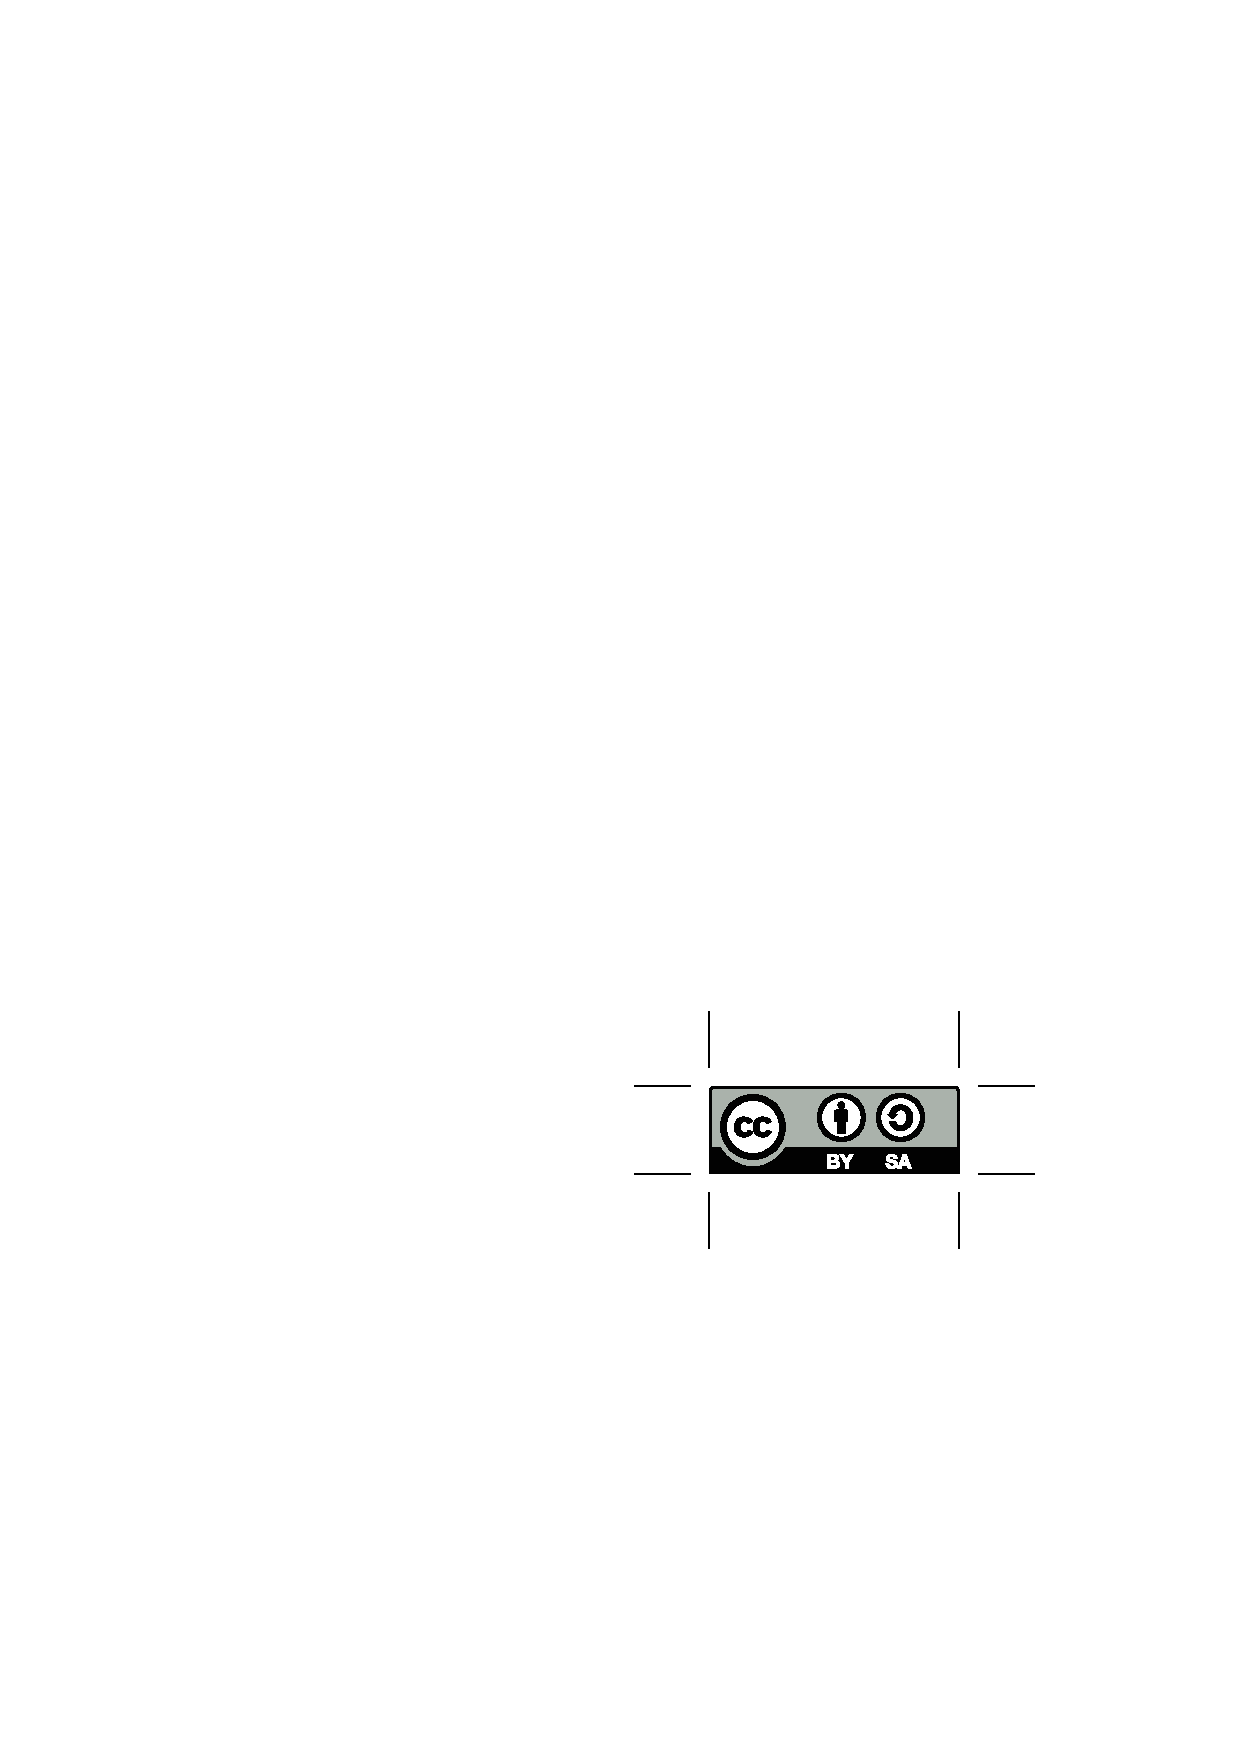
\includegraphics[scale=1]{by-sa} %
    \end{center} %
    
    Este trabajo titulado \emph{\thesisFlatTitle{}} por \thesisAuthor{}, se
    encuentra bajo la Licencia Creative Commons
    \href{http://creativecommons.org/licenses/by-sa/4.0/?ref=chooser-v1}%
    {Atribución-ShareAlike 4.0 International}.
    
    Para ver una copia de esta Licencia, visite
    \url{http://creativecommons.org/licenses/by-sa/4.0/}.\bigskip
    
    \copyright \the\year \hfill%
    \thesisAuthor \hfill%
    \thesisInstitution
  }
}

  
  % Hoja de depuración, con comandos definidos por la plantilla.
  % \phantomsection
\pdfbookmark[1]{Debug}{Debug}

Esta es una página de depuración, para ver todos los comandos
definidos en config.tex

De \verb+babel+ se obtiene que \verb+\tablename+ es \tablename.  Por
lo tanto, en esta versión se usará ``\latabla'' para denotar a cada
``\tabla''.  Ver \tabref{tab:comandostab} para la lista de comandos
existentes.



Este documento es elaborado por \thesisAuthorAddress~\thesisAuthor\
(\thesisAuthorShort) con carné \thesisAuthorTECID, para optar por el
título de \thesisAuthorDegree.

\genderAsesor\ \nameAsesor.

\genderLectorI\ \nameLectorI.

\genderLectorII\ \nameLectorII.

Titulo crudo:

\begin{center}
  \thesisTitle.  
\end{center}

Título aplanado:

``\thesisFlatTitle''.

Palabras clave: \thesisKeywords.

Fecha borrador: \thesisDraftDate

Fecha final: \thesisFinalDate





  
  %\thispagestyle{empty}

\rule{10mm}{0pt}

\vfill

Declaro que el presente documento de tesis ha sido realizado enteramente
por mi persona, utilizando y aplicando literatura referente al tema e
introduciendo conocimientos y resultados experimentales propios.

En los casos en que he utilizado bibliografía he procedido a indicar las
fuentes mediante las respectivas citas bibliográficas.  En consecuencia,
asumo la responsabilidad total por el trabajo de tesis realizado y por
el contenido del presente documento.

\vspace*{8mm}

\begin{flushright}
  \thesisAuthor\par
  Cartago, \FechaFinal\par
  Céd: 1-1741-0734
\end{flushright}

\cleardoublepage

%%% Local Variables: 
%%% mode: latex
%%% TeX-master: "main"
%%% End: 

  %% -------------------------------------------------
  %% Acta y hoja del tribunal
  %%
  %% Asegúrse de que las fechas de defensa de tesis sean las que aparecen
  %% en las actas.
  
  %% Para la Licenciatura en Ingeniería Electrónica:

  %%   Acá se colocan las dos actas como plantillas para ser firmadas
  %%   por el tribunal.

  %%   El acta de aprobación, dependiendo del tribunal, puede dejarla
  %%   en blanco en la tesis, para que el tribunal firme la tesis completa
  %%   sobre esta acta, o, si el tribunal lo decide, extrae la hoja
  %%   para que sea firmada "caligráficamente" por los miembros del tribunal.
  %%   Al acta firmada, en formato PDF (ya sea firmado con tabletas gráficas o
  %%   en papel y escaneada) la integra al documento con el comando para incluir
  %%   el pdf directamente \includepdf{archivo} 
  %%% ESTE ARCHIVO DEBE ELIMINARSE DE LA VERSIÓN FINAL

\thispagestyle{empty}

\begin{center}
  \begin{tabular}{c}
    \thesisInstitution \\
    \thesisDepartment \\
    Trabajo Final de Graduación \\
    Acta de Aprobación
  \end{tabular}
\end{center}

\vfill

\begin{center}
  \begin{tabular}{c}
    Defensa de Trabajo Final de Graduación \\
    Requisito para optar por el título de \thesisAuthorDegree\ en Electrónica\\
    Grado Académico de Licenciatura
  \end{tabular}
\end{center}

\vfill

%% \thesisAuthorAddress, \thesisAuthor y \thesisTitle están en main.tex
El Tribunal Evaluador aprueba la defensa del trabajo final de graduación
denominado \textsl{\thesisFlatTitle{}}, realizado por
%
\thesisAuthorAddress\ \thesisAuthor\ %
%
y, hace constar que cumple con las normas
establecidas por la \thesisDepartment{} del \thesisInstitution{}.

\vfill

\begin{center}
 Miembros del Tribunal Evaluador
\end{center}

\vfill

\begin{center}
  \begin{tabularx}{\textwidth}{cXc}
    \rule{0.45\textwidth}{0.5pt} && \rule{0.45\textwidth}{0.5pt} \\
    \nameLectorI                 && \nameLectorII \\
    \genderLectorI               && \genderLectorII
  \end{tabularx}
  
  \vspace{10mm}

  \begin{tabular}{c}
    \rule{0.45\textwidth}{0.5pt} \\
    \nameAsesor \\
    \genderAsesor
  \end{tabular}
\end{center}

\vfill

\begin{center}
  Cartago, \ifdraft{\thesisDraftDate}{\FechaFinal}\par
\end{center}

\cleardoublepage

%%% Local Variables: 
%%% mode: latex
%%% TeX-master: "main"
%%% End: 
  % Remover en versión final
  %\includepdf{acta_aprob_firmada} % Incluir el acta firmada acá.

  %% El acta de evaluación usualmente la extrae del documento y
  %% la entrega al tribunal para que sea firmada, y ellos la hacen
  %% llegar al profesor del curso de TFG.  Ese documento no
  %% debe aparecer en la tesis final, así que esta línea deberá
  %% comentarla en la versión final:
  %%% ESTE ARCHIVO DEBE ELIMINARSE DE LA VERSIÓN FINAL


\thispagestyle{empty}

\begin{center}
  \begin{tabular}{c}
    \thesisInstitution \\
    \thesisDepartment \\
    Trabajo Final de Graduación \\
    Tribunal Evaluador \\
    Acta de Evaluación
  \end{tabular}
\end{center}

\vfill

\begin{center}
  \begin{tabular}{c}
    Defensa del Trabajo Final de Graduación \\
    Requisito para optar por el título de \thesisAuthorDegree\ en Electrónica\\
    Grado Académico de Licenciatura
  \end{tabular}
\end{center}

\vfill

%% Configurar todo en config.tex
\begin{center}

  Estudiante:%
  \qquad \textbf{\thesisAuthor}%
  \qquad Carné: \thesisAuthorTECID

  \vspace*{2ex}

  \setlength\tabcolsep{0pt}
  \begin{tabular}{p{.25\textwidth}p{.73\textwidth}}
    Nombre del proyecto: & \textsl{\thesisFlatTitle}
  \end{tabular}
\end{center}
\vspace{5mm}

\vfill

Los miembros de este Tribunal hacen constar que este trabajo final de
graduación ha sido aprobado y cumple con las normas establecidas por
la \thesisDepartment{} del \thesisInstitution{} y es merecedor de la
siguiente calificación:

\vfill

\begin{center}
  Nota del Trabajo Final de Graduación: \rule{25mm}{0.5pt}
\end{center}

\vfill

\begin{center}
 Miembros del Tribunal Evaluador
\end{center}

\vfill

% Defina con \setLector* en main.tex (líneas 87-89) los lectores y asesor
\begin{center}
  \begin{tabularx}{\textwidth}{cXc}
    \rule{0.45\textwidth}{0.5pt} && \rule{0.45\textwidth}{0.5pt} \\
    \nameLectorI                 && \nameLectorII \\
    \genderLectorI               && \genderLectorII
  \end{tabularx}
  
  \vspace{10mm}

  \begin{tabular}{c}
    \rule{0.45\textwidth}{0.5pt} \\
    \nameAsesor \\
    \genderAsesor
  \end{tabular}
\end{center}

\vfill

\begin{center}
  Cartago, \ifdraft{\thesisDraftDate}{\thesisFinalDate}\par
\end{center}

\cleardoublepage

%%% Local Variables: 
%%% mode: latex
%%% TeX-master: "main"
%%% End: 
   % >> Remover en versión final <<
    
  %% Para la maestría en electrónica:
  %%% ESTE ARCHIVO DEBE ELIMINARSE DE LA VERSIÓN FINAL

\thispagestyle{empty}

\begin{center}
  \begin{tabular}{c}
    \thesisInstitution \\
    \thesisDepartment \\
    Proyecto de Graduación \\
    Tesis de Maestría \\
    Tribunal Evaluador
  \end{tabular}
\end{center}

\vfill

Tesis de maestría defendida ante el presente Tribunal Evaluador como
requisito para optar por el grado académico de maestría, del
\thesisInstitution.

\vfill

\vspace*{20mm}
\begin{center}
 Miembros del Tribunal
\end{center}
\vspace*{8mm}

\vfill

\begin{center}
  \begin{tabularx}{\textwidth}{cXc}
    \rule{0.45\textwidth}{0.5pt} && \rule{0.45\textwidth}{0.5pt} \\
    \nameLectorI                 && \nameLectorII \\
    \genderLectorI               && \genderLectorII
  \end{tabularx}
  
  \vspace{10mm}

  \begin{tabular}{c}
    \rule{0.45\textwidth}{0.5pt} \\
    \nameAsesor \\
    \genderAsesor
  \end{tabular}
\end{center}

\vfill


Los miembros de este Tribunal dan fe de que la presente tesis de
maestría ha sido aprobada y cumple con las normas establecidas por la
\thesisDepartment.

\vfill

\begin{center}
  Cartago, \today\par
\end{center}

\cleardoublepage

%%% Local Variables: 
%%% mode: latex
%%% TeX-master: "main"
%%% End: 
  % Remover en versión final
  %%% ESTE ARCHIVO DEBE ELIMINARSE DE LA VERSIÓN FINAL


\thispagestyle{empty}

\begin{center}
  \begin{tabular}{c}
    \thesisInstitution \\
    \thesisDepartment \\
    Tesis de Maestría \\
    Acta de Evaluación
  \end{tabular}
\end{center}

\vfill

Tesis de maestría defendida ante el presente Tribunal Evaluador como
requisito para optar por el grado académico de maestría, del
\thesisInstitution.

\vspace*{15mm}

%% Configurar todo en config.tex
\begin{center}
  Estudiante: \thesisAuthor
\end{center}

\vfill

\begin{center}
  Nombre del Proyecto: \thesisFlatTitle}
\end{center}

\vspace*{20mm}
\begin{center}
 Miembros del Tribunal Evaluador
\end{center}
\vspace*{8mm}

\vfill

% Los nombres de lectores y asesor se definen en el archivo main.tex
\begin{center}
  \begin{tabularx}{\textwidth}{cXc}
    \rule{0.45\textwidth}{0.5pt} && \rule{0.45\textwidth}{0.5pt} \\
    \nameLectorI                 && \nameLectorII \\
    \genderLectorI               && \genderLectorII
  \end{tabularx}
  
  \vspace{10mm}

  \begin{tabular}{c}
    \rule{0.45\textwidth}{0.5pt} \\
    \nameAsesor \\
    \genderAsesor
  \end{tabular}
\end{center}

\vfill

Los miembros de este Tribunal dan fe de que la presente tesis de
maestría ha sido aprobada y cumple con las normas establecidas por la
\thesisDepartment.

\vfill

\begin{center}
  Nota final de la Tesis de Maestría: \rule{3cm}{0.5pt}
\end{center}
\vfill

\begin{center}
  Cartago, \today\par
\end{center}

\cleardoublepage

%%% Local Variables: 
%%% mode: latex
%%% TeX-master: "main"
%%% End: 
   % Remover en versión final
  %% -------------------------------------------------
  %\chapter*{Resumen}
\thispagestyle{empty}

El resumen es la síntesis de lo que aparece en el resto del
documento. Tiene que ser lo suficientemente conciso y claro para que
alguien que lo lea sepa qué esperar del resto del trabajo, y se motive
para leerla completamente.  Usualmente resume lo más relevante de la
introducción y contiene la conclusión más importante del trabajo.

Es usual agregar palabras clave, que son los temas principales
tratados en el documento. El resumen queda fuera de la numeración del
resto de secciones.

Evite utilizar referencias bibliográficas, \tablas, o figuras en el
resumen.

\bigskip

%% Defina las palabras clave con defKeywords en config.tex:
\textbf{Palabras clave:} \thesisKeywords

\clearpage
\chapter*{Abstract}
\thispagestyle{empty}

Current advances in network speed, image processing, and digital technology have rendendered live video tools commonplace in professional, academic, and recreational contexts. Therefore, there has been increased interest in ensuring a high quality of experience (QoE) for these services.

Same content as the Spanish version, just in English.  Check
\href{https://deepl.com}{this site} for some help with the
translation.  For instance, the following is the automatic translation
from a previous version of the ``Resumen''.

The abstract is the synthesis of what appears in the rest of the
document. It has to be concise and clear enough so that someone
reading it knows what to expect from the rest of the text, and is
motivated to read it in full.  It usually summarizes the most relevant
parts of the introduction and contains the most important conclusion of
the work.

It is usual to add keywords, which are the main topics covered in the
document. The abstract is left out of the numbering of the rest of the
sections.

Avoid using bibliographical references, tables, or figures in the
abstract.

\bigskip

\textbf{Keywords:} word 1, word 2, 

\cleardoublepage

%%% Local Variables: 
%%% mode: latex
%%% TeX-master: "main"
%%% End: 

  %\vspace*{0.4\textheight}
% No debe confundirse la dedicatoria con el agradecimiento.
% La dedicatoria solo tiene una línea corta de la persona a quien se dedica.

{\hfill{\Large{\emph{Dedicated to family, friends, and all that which keeps us sane}}}}

  %\chapter*{Acknowledgements}
\thispagestyle{empty}

I thank my mom Maritza Badilla, my dad Ricardo Guindon, my sister Hazel, my brother David, the extended Guindon family, and the Monteverde community, which supplied the perfect environment for maximum development in both artistic endeavor and scientific enterprise.

I thank Elena, for sharing her support during the development of this project.

I thank my closest highschool friends Diego, Cristina, and Josue, for stubbornly distracting me from my research. I know you all were acting in my best interests, or so you all say.

I thank my closest college friend Emi, my close friends at the SeleHouse, my friends at Tec, and my friends at RidgeRun, which have all provided spaces where I've shared my research's progress.

I thank Marco Madrigal and Melissa Montero at RidgeRun, for contributing professional management over the dispTec project, as well as providing me with valuable lessons during one of the hardest points in my life.

I thank those brilliant minds I've worked with at RidgeRun, which have trained me in the art of developing all sorts of software shenanigans.

I thank Pablo Alvarado, for contributing his extensive personal expertise, his time and patience, his enthusiasm for understanding, his natural talent as an instructor, his steady push to bring out the most of me, and his nerdy jokes.

\vspace*{1cm}

\thesisAuthor

Cartago, \today

\cleardoublepage

%%% Local Variables: 
%%% mode: latex
%%% TeX-master: "paMain"
%%% End: 


  %----------------------------------------------------------------------------
  \frontmatter
  %----------------------------------------------------------------------------
  \pagestyle{fancy}
  \pagenumbering{roman}

  \pdfbookmark[1]{Indice General}{Indice General}

  \parskip0ex                           % space between paragraphs

  \tableofcontents                      % Table of contents
  \listoffigures                        % List of figures
  \listoftables                         % List of tables

\ifdraft{%
  % todo's                              % TODOs
  \listoftodo
}{%
}

  %%% ---------------------------------------------------------------------------
%% paNotation.tex
%%
%% Notation
%%
%% $Id: paNotation.tex,v 1.15 2004/03/30 05:55:59 alvarado Exp $
%% ---------------------------------------------------------------------------

\cleardoublepage
\renewcommand{\nomname}{List of Symbols and Abbreviations}
\setlength{\nomitemsep}{-\parsep}

%%
% Commands required for the nomenclature groups
%
% There are following prefix forms:
%  a   abbreviation    \syma[key]{symbol}{description}
%  g   general         \symg[key]{symbol}{description}
%%

\renewcommand{\nomgroup}[1]{%
  \ifthenelse{\equal{#1}{G}}{\section*{\hspace*{-\leftmargin}General Notation}}{}%
  \ifthenelse{\equal{#1}{A}}{\section*{\hspace*{-\leftmargin}Abreviations and Acronyms}}{}%
}

\newcommand{\syma}[3][foo]{%
  \ifthenelse{\equal{#1}{foo}}%
  {\nomenclature[A]{#2}{#3}}{\nomenclature[A#1]{#2}{#3}}}
\newcommand{\symg}[3][foo]{%
  \ifthenelse{\equal{#1}{foo}}%
  {\nomenclature[G]{#2}{#3}}{\nomenclature[G#1]{#2}{#3}}}

%%
% Símbolos en la notación general
% (es posible poner la declaración en el texto
%%

\symg[yscalar]{$y$}{Scalar.}
\symg[xvector]{$\vct{x}$}{Vector. \newline\hspace{1mm}%
  $\vct{x}=\left[ x_1 \; x_2 \; \ldots \; x_n \right]^T =
  \begin{bmatrix}
    x_1 \\ x_2 \\ \vdots \\ x_n
  \end{bmatrix}$}

\symg[mmatrix]{$\mat{A}$}{Matrix. \newline\hspace{1mm}%
  $\mat{A} =
  \begin{bmatrix}
    a_{11} & a_{12} & \cdots & a_{1m}\\
    a_{21} & a_{22} & \cdots & a_{2m}\\
    \vdots & \vdots & \ddots & \vdots\\
    a_{n1} & a_{n2} & \cdots & a_{nm}\\
  \end{bmatrix}$}
  \symg[S]{$\set{S}$}{Set.}
  \symg[SN]{$\setN$}{Set of Natural Numbers.}
  \symg[SNE]{$\setN_{8-bit}$}{Set of 8-bit Natural Numbers. }

%%
% Algunas abreviaciones
%%

\syma{QoE}{Quality of Experience}
\syma{CPU}{Central Processing Unit}
\syma{GPU}{Graphics Processing Unit}
\syma{MPEG}{Moving Picture Experts Group}
\syma{PLDA}{Packet Loss Detection Algorithm}
\syma{NSGA-II}{Non-dominated Sorting Genetic Algorithm}
\syma{RDF}{Random Decision Forests}
\syma{VCL}{Video Coding Layer}
\syma{NAL}{Network Abstraction Layer}
\syma{SPS}{Sequence Parameter Set}
\syma{PPS}{Picture Parameter Set}
\syma{RTP}{Real-time Transport Protocol}
\syma{NCA}{Non-Concealed Artifact}
\syma{LSAA}{Low Spatial Activity Artifact}
\syma{HSAA}{High Spatial Activity Artifact}
\syma{TCA}{Temporally-Concealed Artifact}
\syma{PA}{Propagation Artifact}
\syma{RPD}{Random Packet Dropper}
\syma{ML}{Machine Learning}
\syma{SAT}{Summed-Area Table}
\syma{SSAT}{Squared Summed-Area Table}
\syma{ARM}{Acorn RISC Machine}
\syma{ITB}{In-the-Bag}
\syma{OOB}{Out-of-Bag}
\syma{TP}{True Positive}
\syma{TN}{True Negative}
\syma{FP}{False Positive}
\syma{FN}{False Negative}
\syma{dT2}{dispTEC2}
\syma{Art-FD}{Artifact Detector based on Random Decision Forests}
\syma{SIMD}{Singe-Instruction Multiple-Output}

\printnomenclature[20mm]

%%% Local Variables:
%%% mode: latex
%%% TeX-master: "paMain"
%%% End:
                    % Abbreviation

  \parskip1.3ex                         % space between paragraphs

  %----------------------------------------------------------------------------
  \mainmatter
  %----------------------------------------------------------------------------
  % where to look for graphics
  \graphicspath{{./}{./fig/}}
  %\pagenumbering{arab}

  % Main files
  %% ---------------------------------------------------------------------------
%% intro.tex
%%
%% Introduction
%%
%% $Id: intro.tex 1477 2010-07-28 21:34:43Z palvarado $
%% ---------------------------------------------------------------------------

\chapter{Entorno del proyecto}
\label{chp:entorno}

La pandemia reciente de COVID-19 ejemplificó el papel de los servicios de video conferencia y de streaming en vivo en la sociedad actual.
Los avances actuales en la velocidad de redes y en la tecnología digital han permitido que estos servicios sean comunes en contextos profesionales, académicos y recreativos.
Por lo tanto, ha aumentado el interés en asegurar una alta calidad de experiencia (QoE, por sus siglas en inglés) para estos servicios.

Uno de los problemas principales que afecta el QoE de los servicios de video conferencia y streaming en vivo son los artefactos de video, como se menciona en \cite{Vranjes2018, Korhonen2018}.
En \cite{Greengrass2009}, los artefactos de video, o simplemente artefactos, se definen como distorsiones en las imágenes desplegadas al usuario con respecto a las imágenes originales capturadas.
Según \cite{Vranjes2018}, los artefactos son causados principalmente por errores o pérdida de datos en la transmisión del video a través de la red, o por pérdidas causadas durante la compresión del video. En la Figura \ref{fig:1.1} se comparan dos versiones de una misma imagen. La Figura \ref{fig:1.1.a} no contiene artefactos de video y la Figura \ref{fig:1.1.b} contiene artefactos de video por pérdida de paquetes.

\begin{figure} [!h]
  \centering
  
  \begin{subfigure}[t]{0.49\textwidth}
    \centering
    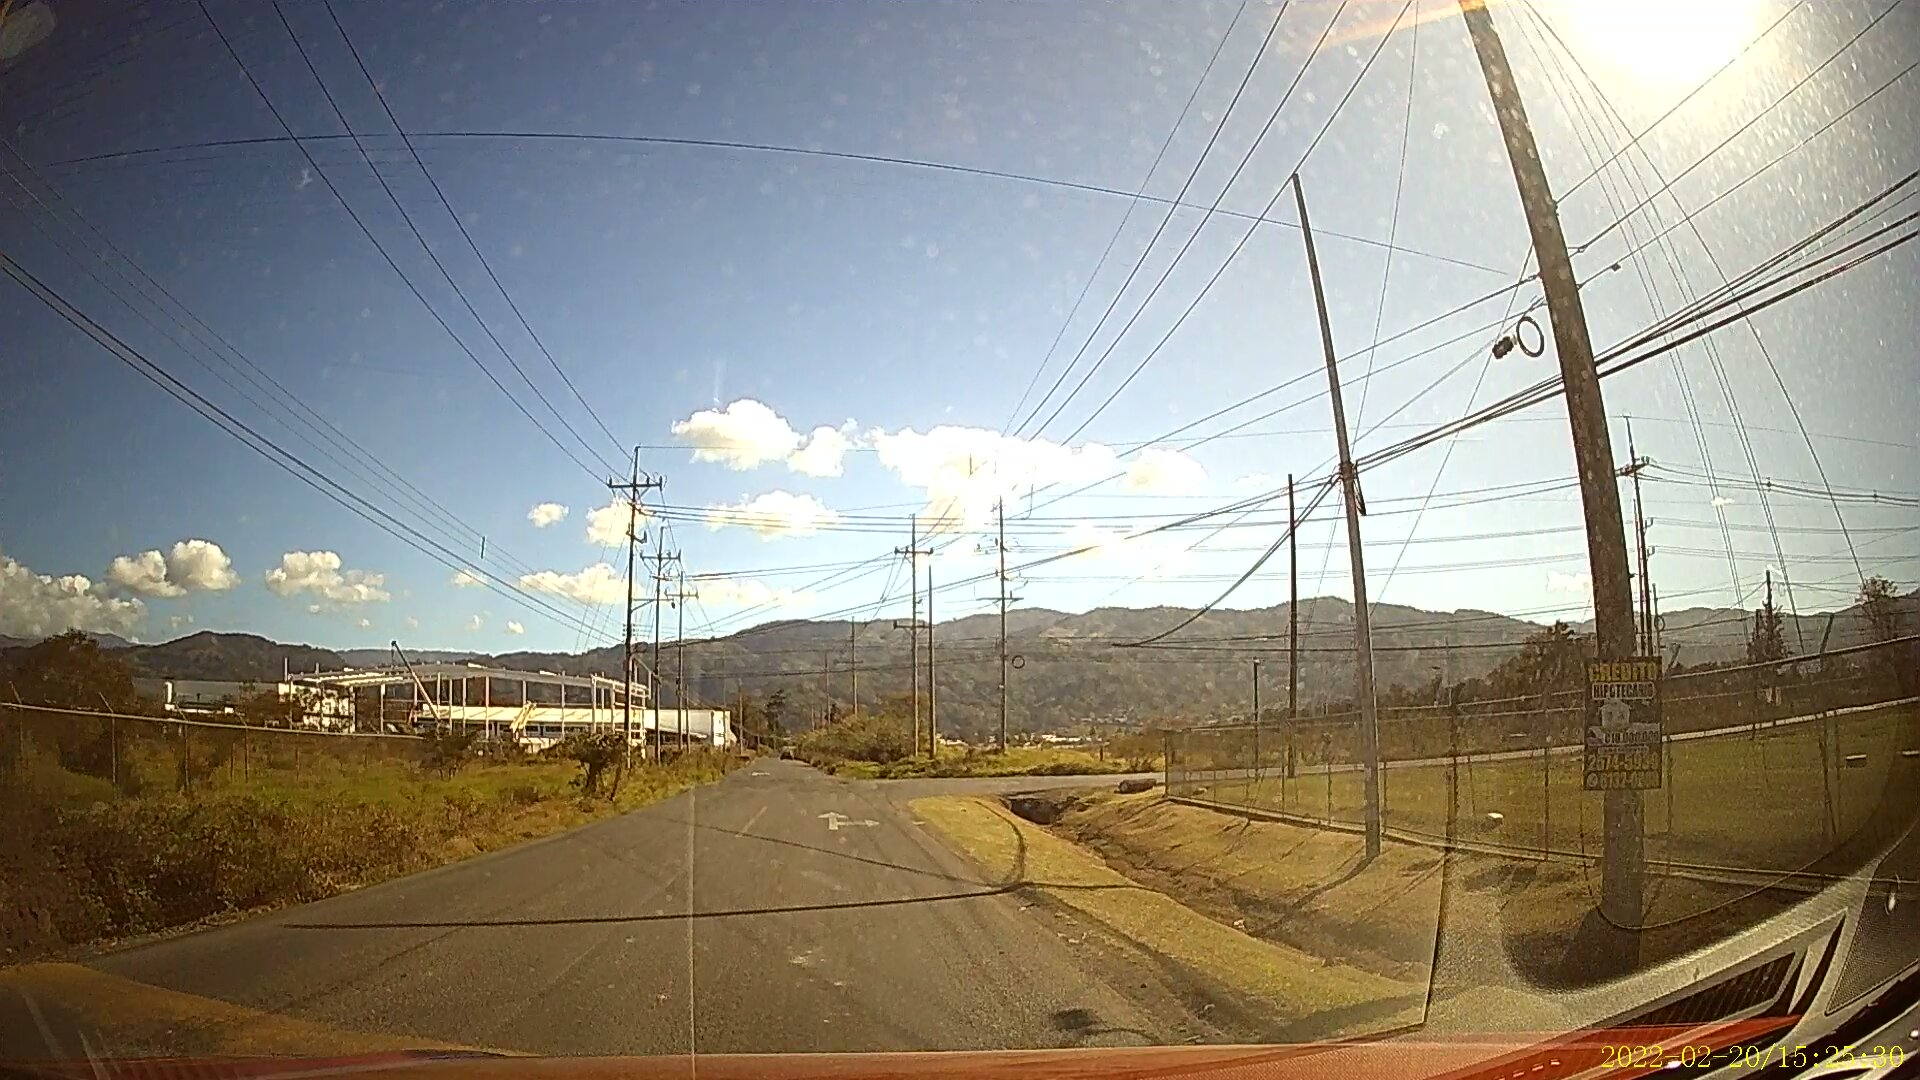
\includegraphics[width=\textwidth]{imgs_27}
    \caption{Cuadro sin pérdida de paquetes}
    \label{fig:1.1.a}
  \end{subfigure}
  \hfill
  \begin{subfigure}[t]{0.49\textwidth}
    \centering
    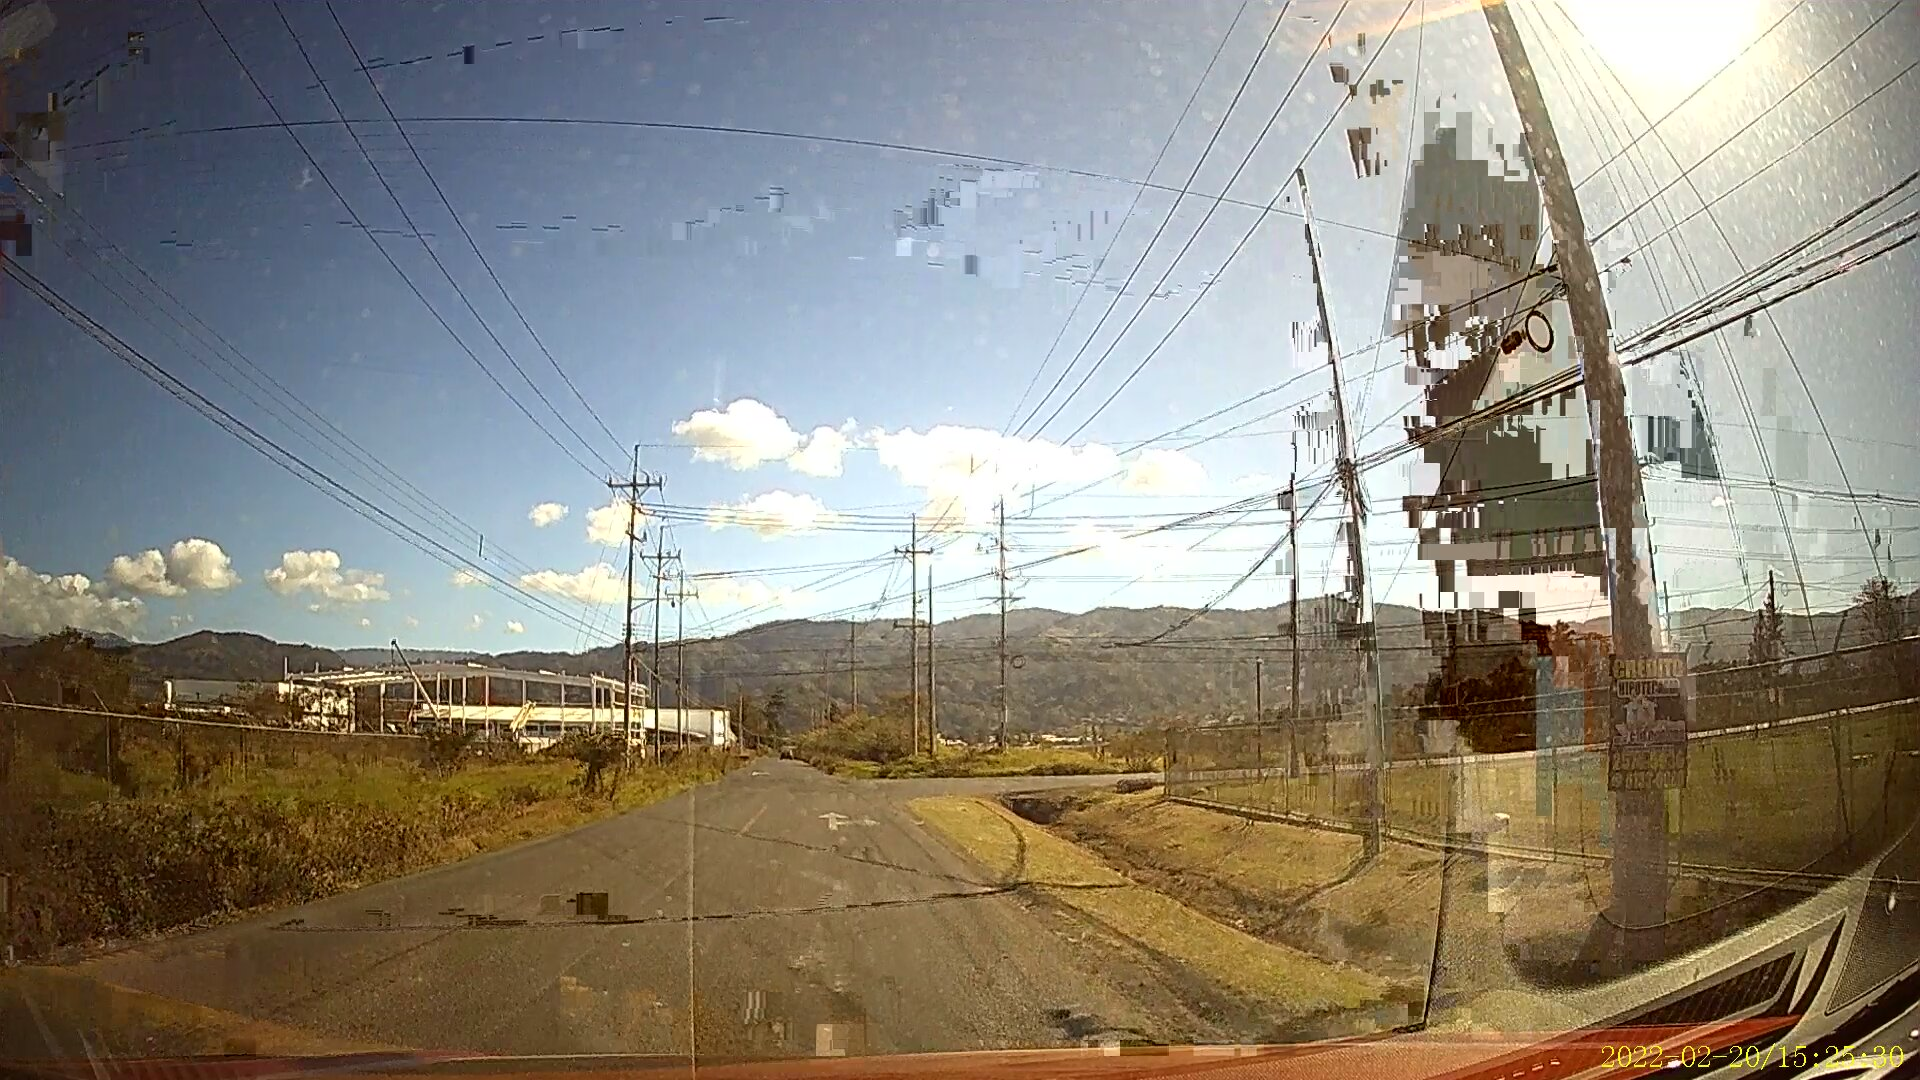
\includegraphics[width=\textwidth]{imgs_with_loss_27}
    \caption{Cuadro con artefactos causados por pérdida de paquetes}
    \label{fig:1.1.b}
  \end{subfigure}
  
  \caption{Ejemplo de artefactos causados por pérdida de paquetes}
  \label{fig:1.1}

\end{figure}

Existen métodos para solucionar los errores de transmisión en la capa de transporte o hasta en la capa de sintaxis de video, como se menciona en \cite{Sanyal2021}.
En estos casos se cuenta con información de cómo están codificados los paquetes de video, por lo cual se simplifica la tarea de detección y corrección de errores.
Cuando el usuario solo cuenta con la información decodificada y descomprimida, es necesario usar métodos para detección y corrección de artefactos que solo cuentan con la información pura de video, como los de \cite{Vranjes2018, Sanyal2021,Goodall2019}.
A estos métodos se le denominan ``métodos sin referencia''.

Los artefactos de video resultan en pérdidas de información del video original. En aplicaciones de video conferencia y streaming en vivo no es posible recuperar la información perdida sin afectar el QoE del usuario.
Para lograr corregir los artefactos de video, los métodos sin referencia deben inferir la información perdida.
Al proceso de restaurar zonas desconocidas de una imagen se le llama ``restauración de video'' \cite{Li2022, Zhou2021}.
La restauración de video, o simplemente restauración, se utiliza comunmente para eliminar la presencia de objetos en un video o una imagen, pero se pueden utilizar para reconstruir zonas de una imagen afectadas por artefactos de video, como se hace en \cite{Dong2023, Brenes2022}.

Los algoritmos modernos de restauración utilizan modelos de aprendizaje de máquina.
Los restauradores de \cite{Li2022, Zhou2021, Liu2021} utilizan ``transformers''.
Los transformers son modelos de aprendizaje de máquina con resultados extraordinarios para tareas de reconstrucción de señales, pero son caros tanto en tiempo como en capacidad de procesamiento \cite{Liu2021}.
Para lograr optimizar el desempeño de estos modelos, se requiere del uso de aceleradores de hardware, el más común siendo el GPU.

Modelos de restauración como el de \cite{Li2022} requiren de máscaras binarias para identificar las zonas que se desea reconstruir.
Por esta razón, se debe detectar la ubicación de los artefactos de video y generar máscaras binarias para luego ser utilizadas en la etapa de reconstrucción de la imagen.

Existen clasificaciones de los distintos tipos de artefactos por pérdida de paquetes \cite{Greengrass2009, Glavota2016}. Estos estudios describen las propiedades estadísticas de los artefactos de video. Por ejemplo, ciertos artefactos de video tienden a tener bordes verticales y horizontales de alto contraste que pueden ser detectados por filtros pasa-altos. En los estándares de compresión de video MPEG y H.26x, los pixeles de una imagen se agrupan en ``macrobloques'', cuales son de grupos de $16 \times 16$ pixeles en la imagen. Pérdidas de paquetes que contienen información de macrobloques resultan en artefactos con bordes bien definidos \cite{Vranjes2019, Glavota2018}.

Los métodos para la detección de artefactos de video de \cite{Vranjes2018, Glavota2018} se centran en algoritmos de filtrado que no involucran aprendizaje de máquina. Estos métodos pueden llegar a procesar más de 30 cuadros de video por segundo contando con solo recursos de CPU, pero sobresimplifican las características de los artefactos de video y no logran alcanzar altas tasas de detección. También existen métodos de detección de artefactos que utilizan redes neuronales, como los de \cite{Goodall2019, Rajasekar2020}. Estos métodos generalizan mejor que los algoritmos de filtrado, pero son más pesados en recursos y requieren de aceleradores, como los GPU, para alcanzar velocidades comparables a los algoritmos de filtrado.

Durante el 2022, el SIPLab desarrolló el proyecto dispTEC2-2022 en conjunto con la empresa RidgeRun para la restauración de video con artefactos por pérdida de paquetes. El proyecto se desarrolló sobre la Jetson TX2 de Nvidia. Este sistema cuenta con un GPU de 256 núcleos CUDA, 4 CPU ARM y 2 CPU Denver. En \cite{Brenes2022} se detalla el desarrollo de la etapa de reconstrucción de imágenes de dispTEC2-2022. Este modelo utiliza el GPU por completo. El modelo de reconstrucción de Brenes requiere de máscaras binarias para ubicar los artefactos en las imágenes de entrada y el proyecto en general carece aún de un método de detección de artefactos.

  %% ---------------------------------------------------------------------------
%% intro.tex
%%
%% Introduction
%%
%% $Id: intro.tex 1477 2010-07-28 21:34:43Z palvarado $
%% ---------------------------------------------------------------------------

\chapter{Planteamiento del problema}
\label{chp:planteamiento}

Un objetivo de la corrección de artefactos de video en aplicaciones de video conferencia y streaming en vivo es asegurar una alta QoE para el usuario final. Además, la corrección de artefactos de video cuenta con una etapa de detección de artefactos y otra etapa de restauración de zonas afectadas. El compromiso entre el costo computacional de estos procesos y los requisitos de QoE para el usuario final complica el desarrollo de un sistema de corrección de artefactos de video.

Se deben establecer criterios de calidad para determinar si el proceso de corrección de artefactos tiene un rendimiento adecuado. La calidad percebida por el usuario final depende por lo menos de dos criterios: la velocidad del video final y la calidad de imagen en el video final.

Para determinar un criterio de velocidad de video apropiada, se considera Zoom como ejemplo de una aplicación de video conferencia. Según \cite{ZoomSupport}, Zoom recomienda utilizar la aplicación a una resolución de $1280 \times 720$ pixeles y a 30 cuadros por segundo. Bajo esta recomendación, un obstáculo al que se enfrenta el procesamiento de detección y restauración de artefactos, es de lograr operar sobre cuadros de $1280 \times 720$ pixeles a una velocidad de 30 cuadros por segundo. En términos de tiempo de procesamiento, cada cuadro debe ser procesado en alrededor de 33 ms. Para fines de este documento, se le refiere a esta velocidad de procesamiento como ``tiempo real''.

Para cada cuadro, es necesario detectar las ubicaciones de los artefactos de video y luego realizar el proceso de restauración. Para que el procesamiento total suceda a tiempo real, tanto la etapa de detección como la etapa de restauración deben durar aún menos tiempo que 33 ms por cuadro.

El procesamiento de restauración, que depende del uso de redes neuronales, requiere el uso de aceleración por hardware para lograr procesar en tiempo real \cite{Li2022}. Por lo tanto, se deben tomar en cuenta los recursos disponibles en el equipo sobre el cual se realiza la corrección de artefactos de video.

Si la corrección de los artefactos de video suceden en un mismo equipo, el proceso de detección debe compartir recursos con el proceso de restauración. Tomando en cuenta que el proceso de restauración require de un acelerador, se debe considerar que los recursos disponibles para el proceso de detección son limitados.

La calidad del video final depende tanto de la efectividad del proceso de detección, como de la capacidad del proceso de restauración. La efectividad del proceso de detección se puede medir a través de las métricas de precisión y exhaustividad. Utilizando las definiciones de \cite{ScikitLearn}, precisión es la proporción entre la cantidad de detecciones correctas y la cantidad de detecciones totales. Exhaustividad es la proporción entre la cantidad de detecciones correctas y la cantidad de detecciones que idealmente se deben obtener. Para asegurar una alta calidad de detección de artefactos, se deben considerar los criterios de precisión y exhaustividad del método de detección.

La complejidad algorítmica del método de detección directamente afecta la capacidad de procesamiento que se requiere para realizar la detección. Los recursos disponibles para la detección afectan tanto la velocidad como la capacidad de procesamiento disponible para la detección. Por lo tanto, se debe considerar el compromiso entre recursos disponibles, velocidad de la detección y calidad de la detección.

El trabajo de \cite{Brenes2022} realiza el proceso de restauración de imágenes y ejecuta sobre una Nvidia Jetson TX2. Para ejecutar utiliza el GPU por completo. Este trabajo carece de un detector de artefactos para identificar las zonas de la imagen que se deben restaurar.

  %% ---------------------------------------------------------------------------
%% intro.tex
%%
%% Introduction
%%
%% $Id: intro.tex 1477 2010-07-28 21:34:43Z palvarado $
%% ---------------------------------------------------------------------------

\chapter{Síntesis del problema}
\label{chp:sintesis}

No existe un método de detección de artefactos de video para ser utilizado en restauración de video en tiempo real que considere el compromiso entre la administración de recursos disponibles en el equipo a emplear, la velocidad a tiempo real que se desea alcanzar y la calidad del método de detección.

  %% ---------------------------------------------------------------------------
%% intro.tex
%%
%% Introduction
%%
%% $Id: intro.tex 1477 2010-07-28 21:34:43Z palvarado $
%% ---------------------------------------------------------------------------

\chapter{Enfoque de la solución}
\label{chp:enfoque}

La elección de un método de detección de artefactos de video está delimitado por las siguientes consideraciones:
\begin{enumerate}
    \item Se debe lograr detectar la ubicación de los artefactos de video considerando la precisión y exhaustividad que se desean alcanzar
    \item Se debe optimizar el uso de recursos del equipo a utilizar, ya que el proceso de detección debe correr junto al proceso de restauración de imágenes.
    \item Se debe optimizar la velocidad del método de detección para permitir que el sistema de corrección pueda ejecutarse en tiempo real
\end{enumerate}

\section{Posibles soluciones}

\begin{enumerate}
    \item Una posible solución al problema es de implementar un algoritmo a base de filtrado de imágenes. Como se menciona en \cite{Vranjes2018, Glavota2018}, es posible aprovechar características estadísticas de los artefactos para lograr determinar sus ubicaciones. Estos algoritmos ofrecen ventajas en términos de su capacidad de correr con pocos recursos y permitir ejecución en tiempo real. El problema con estos algoritmos es que no consideran la variedad de irregularidades en la naturaleza de los artefactos de video, por lo cual no alcanzan niveles altos de detección. Además, estos métodos cuentan con parámetros para ajustar el comportamiento del filtrado que deben ser ajustados a mano, por lo cual tienen configuraciones dependentientes de cada situación.

    \item Otra posible solución al problema es implementar y entrenar una red neuronal que recibe las imágenes de entrada y genere máscaras de salida con las ubicaciones de los artefactos detectados. Estos métodos se utilizan en \cite{Goodall2019,Rajasekar2020}. Las redes neuronales son algoritmos que aprenden a partir de un conjunto de datos de entrenamiento a generalizar la detección de errores con datos de prueba con los cuales no se ha entrenado. Las redes neuronales alcanzan altos niveles de detección, pero requieren de GPU para correr en tiempo real.

    \item Una tercer posible solución al problema es implementar y entrenar un Bosque de Decisión Aleatoria que reciba cierta información sobre el macrobloque de una imagen sobre la cual se desea realizar la detección y decida si tiene o no tiene un error. Estos algoritmos logran altos niveles de detección, pero además tienen la ventaja de ser computacionalmente muy eficientes tanto en recursos como en tiempo de ejecución \cite{Keskin2012}.
\end{enumerate}

\section{Selección de la solución}

La solución más adecuada al problema de detección de artefactos de video es la implementación de un Bosque de Decisión Aleatoria. Los bosques tienen ventajas sobre las otras posibles soluciones dadas las limitaciones de velocidad, recursos y calidad que se deben considerar. Los algoritmos de filtrado son eficientes en uso de recursos y son veloces, pero están limitados en su habilidad de generalizar a una gran variedad de artefactos, por lo cual no cuentan con la mejor calidad de detección. Las redes neuronales son algoritmos poderosos y resultan en los mejores resultados de detección, pero consumen más recursos de los que se disponen para la detección de artefactos. Si se ejecutan las redes neuronales con recursos limitados, el tiempo de procesamiento aumenta considerablemente. Los bosques de decisión aleatoria son capaces de generalizar tareas de detección con imágenes \cite{Keskin2012}, además de ser eficientes en usos de recursos y velocidad. Por esta razón los Bosques de Decisión Aleatoria son la solución más apropiada para el problema a solucionar.

La Tabla \ref{tab:sel_sol} es una Matriz de Pugh que compara criterios, con tal de demostrar que entre las soluciones propuestas, la implementación de un Bosque de Decisión Aleatoria es la eleción más apropiada. Dos criterios considerados son el consumo de memoria y de CPU. Para la corrección de artefactos de video, el proceso de detección de artefactos debe compartir recursos con el proceso de reconstrucción de imágenes. Además el proceso de reconstrucción debe contar con un acelerador para lograr ejecutarse en tiempo real. Por lo tanto, la elección del método de detección de artefactos debe considerar un uso limitado de recursos. La efectividad de la solución, y en particular la métrica de exhaustividad de la solución determina si la solución es viable. La velocidad que logra alcanzar cada solución se relaciona inversamente con la complejidad algorítmica. El proceso de detección de artefactos debe ejecutarse en tiempo real, por lo cual debe utilizar un algoritmo veloz. La complejidad de implementación determina si la solución es factible de desarrollarse en el periodo establecido para la ejecución del proyecto.

\begin{table} [!h]
    \caption{Matriz de Pugh para la selección de solución}
    \label{tab:sel_sol}
    \centering
    \begin{tabular}{p{3.5 cm} p{2.5 cm} p{2.5 cm} p{3.5 cm}}
        \hline
        Criterios & Algoritmo de Filtrado & Red neuronal & Bosque de decisión aleatoria \\
        \hline
        Consumo memoria & 0 & -1 & 0 \\
        Consumo CPU & 1 & -1 & 1 \\
        Efectividad & -1 & 1 & 1 \\
        Velocidad & 1 & -1 & 1 \\
        Implementación & 0 & 0 & -1 \\
        \hline
        Total & 1 & -1 & 2 \\
        \hline
        Prioridad & 2 & 3 & 1 \\
        \hline
    \end{tabular}
\end{table}

\newpage

La solución debe evaluarse variando las condiciones de captura. En la Tabla \ref{tab:base_de_datos} se resumen los criterios para el conjunto de datos con el que se debe probar la solución.

\begin{table} [!h]
    \caption{Criterios para base de datos de prueba}
    \label{tab:base_de_datos}
    \centering
    \begin{tabular}{l c}
        \hline
        Criterios & Cantidad \\
        \hline
        Categorías de actividades & 6 \\
        Condiciones de luz & 3 \\
        Tamaño mínimo de cada video (cuadros) & 600 \\
        Resolución mínima de cada video (pixeles) & $1280 \times 720$ \\
        \hline
    \end{tabular}
\end{table}

  %% ---------------------------------------------------------------------------
%% intro.tex
%%
%% Introduction
%%
%% $Id: intro.tex 1477 2010-07-28 21:34:43Z palvarado $
%% ---------------------------------------------------------------------------

\chapter{Objetivos}
\label{chp:objetivos}

\section{Objetivo general}

Desarrollar un sistema para la detección y localización de errores por pérdida de paquetes en imágenes de un video codificado con H264 en tiempo real, utilizando solo los recursos de CPU de la Jetson TX2 de NVIDIA, mediante un Bosque de Decisión Aleatoria.

Indicador: Las métricas de precisión y exhaustividad deben ser mayores a 70\%. La duración de detección menor a 33 ms, y el perfil de uso de recursos debe mostrar el uso exclusivo de CPU.

Entregable: Sistema de detección que recibe imágenes con errores por pérdida de paquetes y produce máscaras binarias con los resultados de detección de errores.

\section{Objetivos Específicos}

\begin{enumerate}
    \item Generar el conjunto de datos de entrenamiento y prueba que contenga videos base, con variedad de escenas y colores, los videos correspondientes con errores de pérdida de paquetes generados, junto a datos de referencia que indican las ubicaciones de los errores generados.

    Indicador:  El conjunto de datos cumple con los criterios expuestos en la Tabla \ref{tab:base_de_datos}, acompañados por su versión con errores generados y sus datos de referencia que indica las ubicaciones de los errores generados.

    Entregable: El conjunto de datos.

    \item Diseñar e implementar un Bosque de Decisión Aleatoria mediante el conjunto de datos generado para lograr metricas de precisión y exhaustividad mayores a 70\%.

    Indicador: Las métricas de precisión y exhaustividad deben ser mayores a 70\% con un conjunto de prueba con el cual no ha sido entrenado.

    Entregable: El modelo de bosque de decisión aleatoria entrenado.

    \item Optimizar Bosque de Decisión Aleatoria para lograr ejecutar detección en tiempo real de artefactos en una imagen.

    Indicador: El modelo mantiene las métricas de precisión y exhaustividad mayores al 70\% y adicionalmente indica las ubicaciones de los errores en imágenes en menos de 33 ms por imagen.

    Entregable: Un perfil del tiempo de ejecución del modelo

\end{enumerate}
  %% ---------------------------------------------------------------------------
%% intro.tex
%%
%% Introduction
%%
%% $Id: intro.tex 1477 2010-07-28 21:34:43Z palvarado $
%% ---------------------------------------------------------------------------

\chapter{Actividades}
\label{chp:actividades}

Para entrenar y optimizar un bosque de decisión aleatoria que realice detección de artefactos de videos, es necesario iniciar con tareas de investigación y preparación del conjunto de datos. Es necesario investigar las características de los artefactos de video y de los métodos de extracción de características para entrenar bosques de decisión aleatoria. Además es necesario investigar los marcos de trabajo bajo los cuales se desarrollan y optimizan bosques de decisión aleatoria. Se deben investigar las posibles optimizaciones en el hardware a utilizar, pero la mayoría de las tareas de optimización dependen de primero entrenar un bosque que realice la detección de artefactos.

La Tabla \ref{tab:actividades} resume las actividades a desarrollar, además de sus requisitos y los objetivos a los cuales corresponden.

\begin{table} [!h]
    \caption{Actividades a realizar, organizadas por objetivo e indicando sus respectivos requisitos y duraciones (en días)}
    \label{tab:actividades}
    \centering
    \begin{tabular}{p{0.4 cm} p{7.8 cm} p{1.6 cm} p{2 cm} p{2 cm}}
        \hline
        $\#$ & Actividad & Objetivo & Requisitos & Duración \\
        \hline
        1 & Coleccionar videos a utilizar como conjunto de datos & 1 & - & 2 \\
        2 & Simular pérdida de paquetes sobre conjunto de datos & 1 & 1 & 1 \\
        3 & Generar datos de referencia comparando datos con pérdidas y datos originales & 1 & 2 & 2 \\
        \hline
        4 & Investigar características de artefactos de video por pérdida de paquetes & 2 & - & 10 \\
        5 & Investigar estrategias de extracción de características para bosques de decisión aleatoria orientados a imágenes & 2 & - & 10 \\
        6 & Investigar marcos de trabajo para entrenar bosques de decisión aleatoria & 2 & - & 10 \\
        7 & Determinar estrategias de extracción de características sobre datos con pérdidas & 2 & 4, 5 & 5 \\
        8 & Determinar e instalar marco de trabajo para entrenar bósques de decisión aleatoria & 2 & 6 & 5 \\
        9 & Entrenar bosques & 2 & 3, 7, 8 & 20 \\
        \hline
        10 & Investigar estrategias de optimización por software para estrategias de extracción de características & 3 & 5 & 25 \\
        11 & Investigar estrategias de optimización por hardware para la Jetson TX2 & 3 & - & 25 \\
        12 & Implementar estrategias de optimización sobre extracción de características & 3 & 9, 10, 11 & 20 \\
        \hline
    \end{tabular}
\end{table}

  %% ---------------------------------------------------------------------------
%% intro.tex
%%
%% Introduction
%%
%% $Id: intro.tex 1477 2010-07-28 21:34:43Z palvarado $
%% ---------------------------------------------------------------------------

\chapter{Diagramas de Gantt y PERT}
\label{chp:diagramas}

Se inicia el proyecto con las tareas de investigación. A partir de la investigación se determina qué marco de trabajo utilizar para entrenar el bosque de decisión aleatoria y qué estrategias de extracción de características usar para entrenar el bosque. Luego se diseña e implementa el bosque, cual se espera que dure varias semanas para lograr cumplir con los requisitos de calidad requeridos. Finalmente las tareas de optimización se realizan cuando se termine de entrenar el bosque. El Diagrama de Gantt mostrado en la Figura \ref{fig:gantt} ilustra la distribución de actividades en el tiempo. Además, se resalta la ruta crítica del proyecto. Las tareas se inician a partir del 6 de Febrero y se esperan que vayan concluyendo para la última semana de Abril.

\begin{figure} [!h]
    \centering
    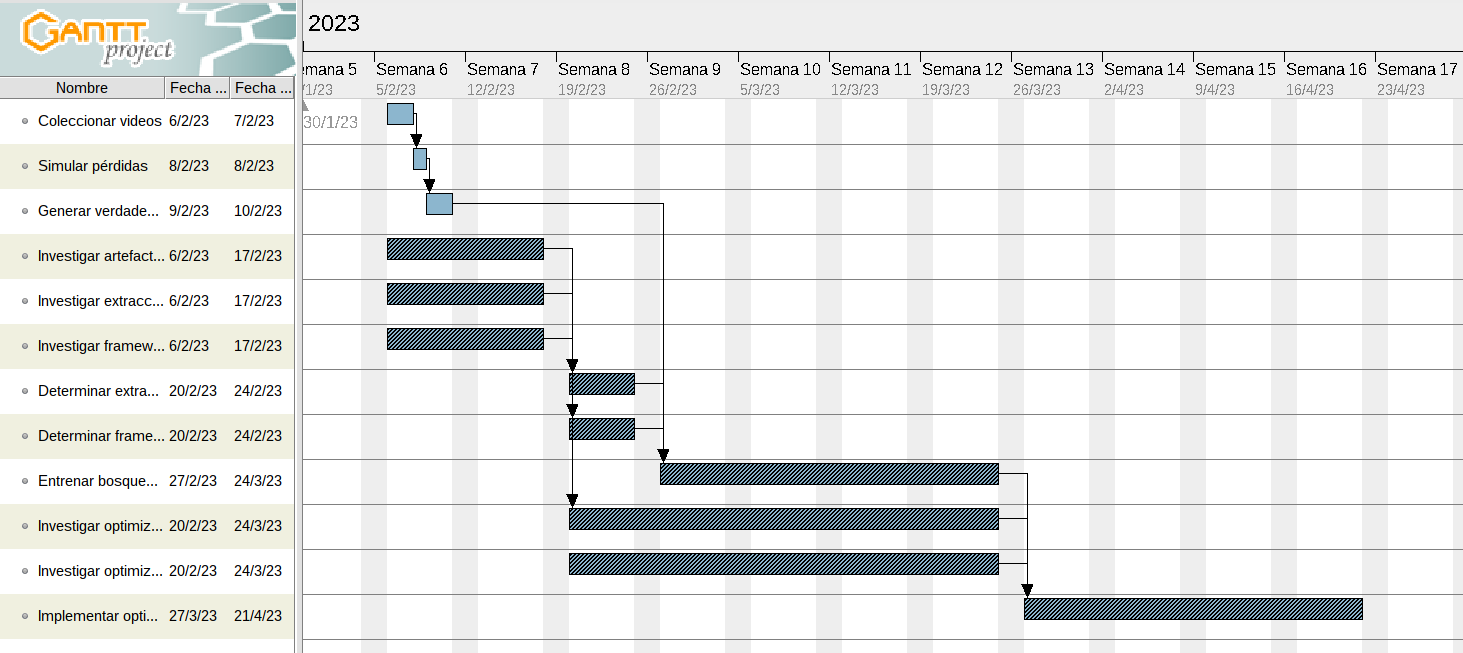
\includegraphics[width=\textwidth]{gantt.png}
    \caption{Diagrama de Gantt}
    \label{fig:gantt}
\end{figure}

El siguiente Diagrama de PERT ilustra la relación de dependencias entre las
actividades a realizar.

\begin{figure} [!htb]
    \centering
    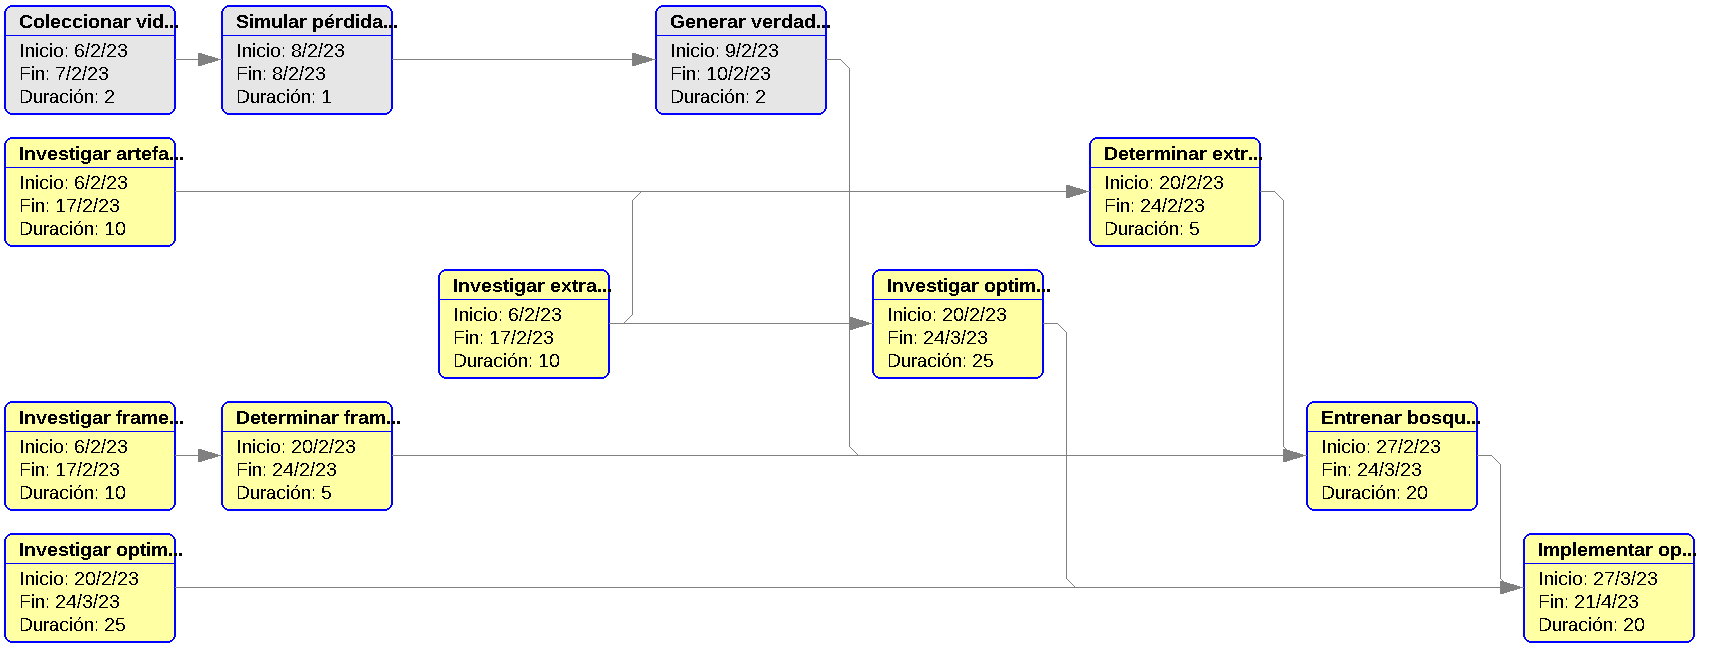
\includegraphics[width=\textwidth]{pert.png}
    \caption{Diagrama de PERT}
    \label{fig:pert}
\end{figure}

El presupuesto del proyecto se muestra en la Figura \ref{fig:presupuesto} y el aporte mensual de la empresa se muestra en la Figura \ref{fig:mensual}.

Como recurso principal del proyecto, se utiliza una de las Nvidia Jetson TX2 del SIPLab de la Escuela de Electrónica del Tec. Para entrenar los modelos, es necesario contar con amplia RAM para lograr cargar los datos de entrenamiento. El Servidor de la Escuela de Electrónica cuenta con una máquina virtual con el sistema operativo Ubuntu 22.04 instalado y 64 Gb de RAM para este propósito. Para el desarrollo de los algoritmos y pruebas, se utiliza una máquina personal.

\begin{figure} [!htb]
    \centering
    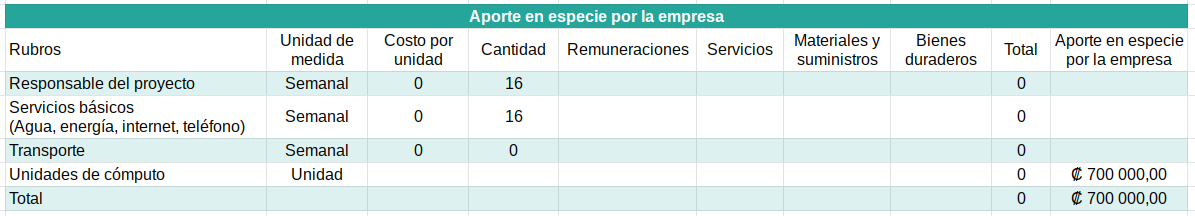
\includegraphics[width=\textwidth]{presupuesto.png}
    \caption{Presupuesto del proyecto}
    \label{fig:presupuesto}
\end{figure}

\begin{figure} [!htb]
    \centering
    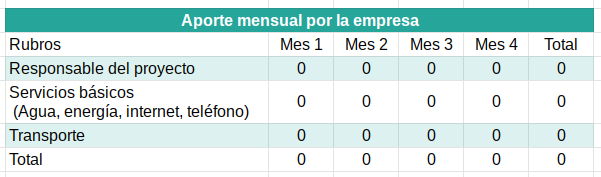
\includegraphics[width=0.5\textwidth]{mensual.png}
    \caption{Aporte mensual de la empresa}
    \label{fig:mensual}
\end{figure}


  %----------------------------------------------------------------------------
  % literature in bibtex way:
  % \bibliographystyle{sty/plainurl} % for english documents
  % \bibliography{literatura}
  % literature in biblatex/biber way
  \printbibliography[title={Bibliografía},heading=bibintoc]
  %----------------------------------------------------------------------------

  %----------------------------------------------------------------------------
  \appendix
  %----------------------------------------------------------------------------

  \chapter{Anexos}
\label{apx:apendice}
\textbf{Exposición de anteproyecto:} \url{https://www.youtube.com/watch?v=7vysEp_0tss}
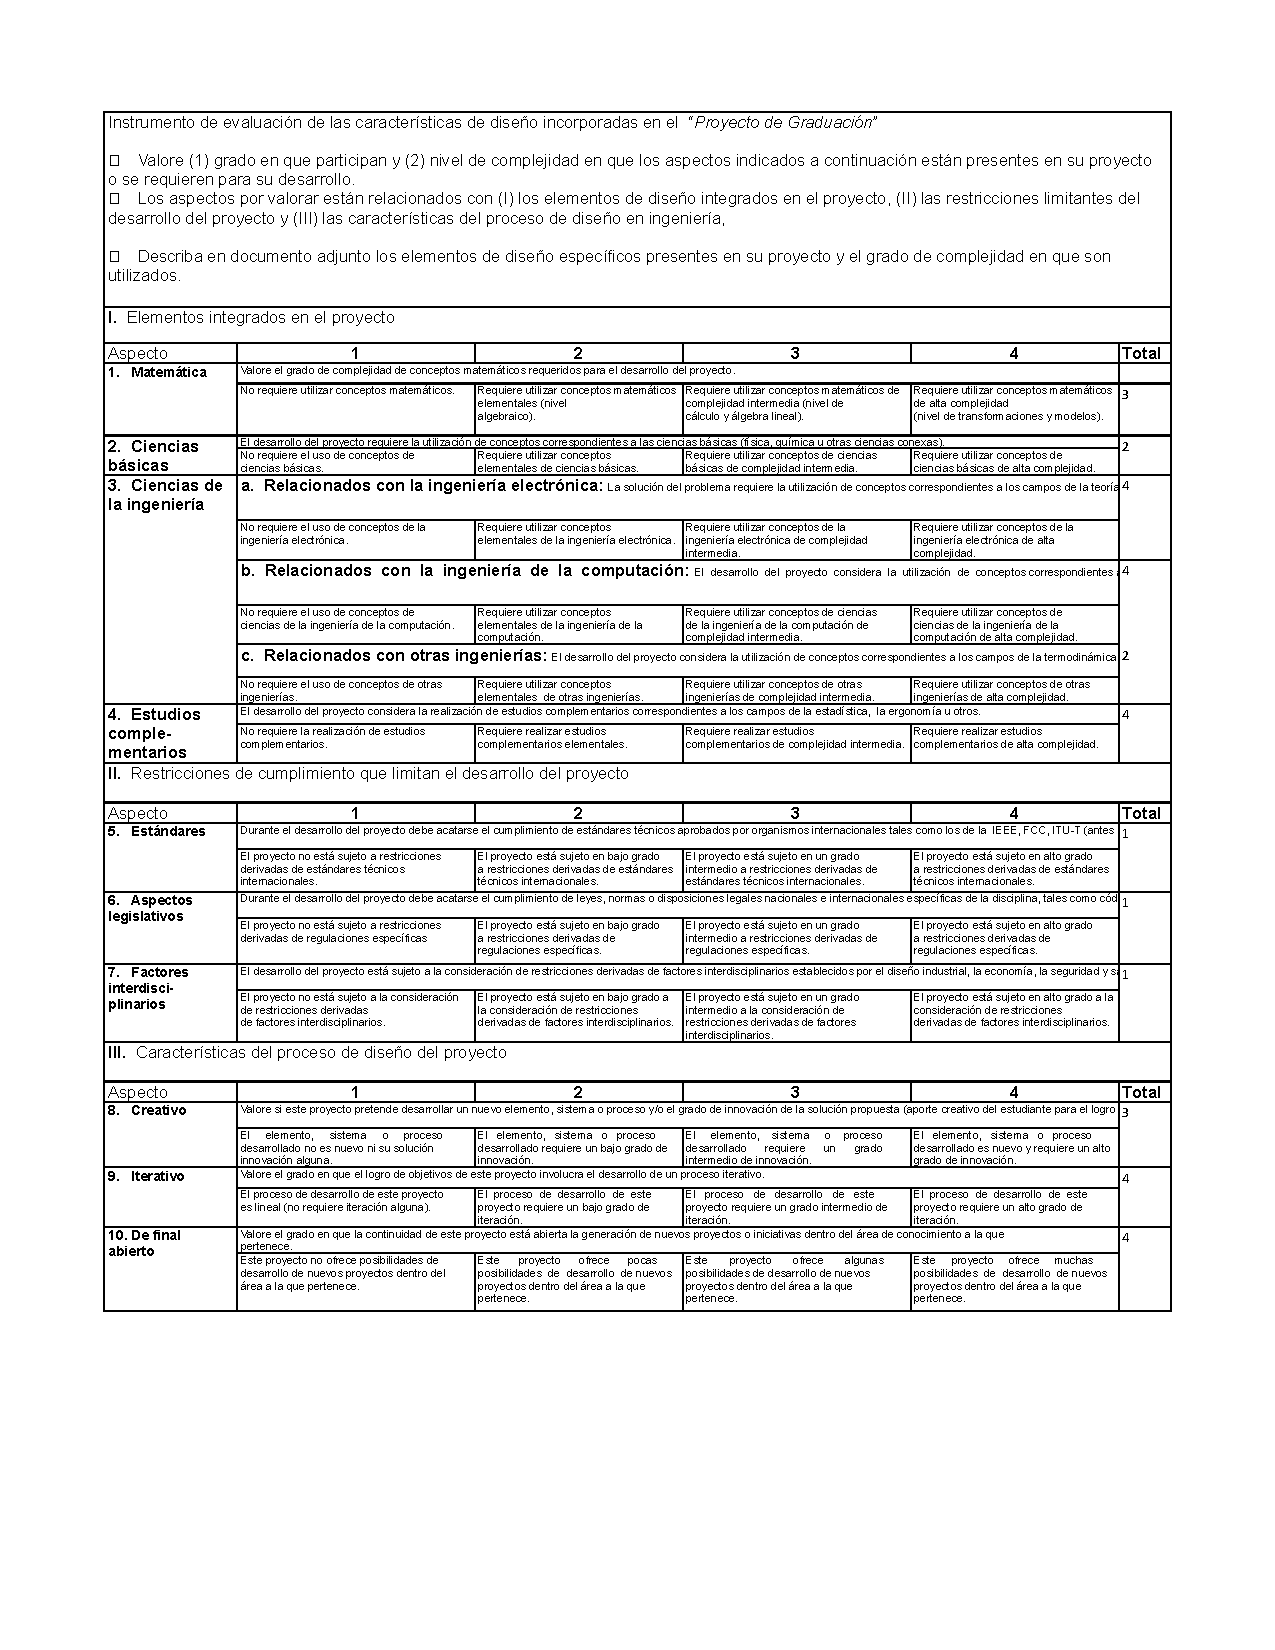
\includepdf[scale=1, offset=3cm -4cm, pagecommand={\textbf{Anexo A}}]{caracteristicas_proceso.pdf}
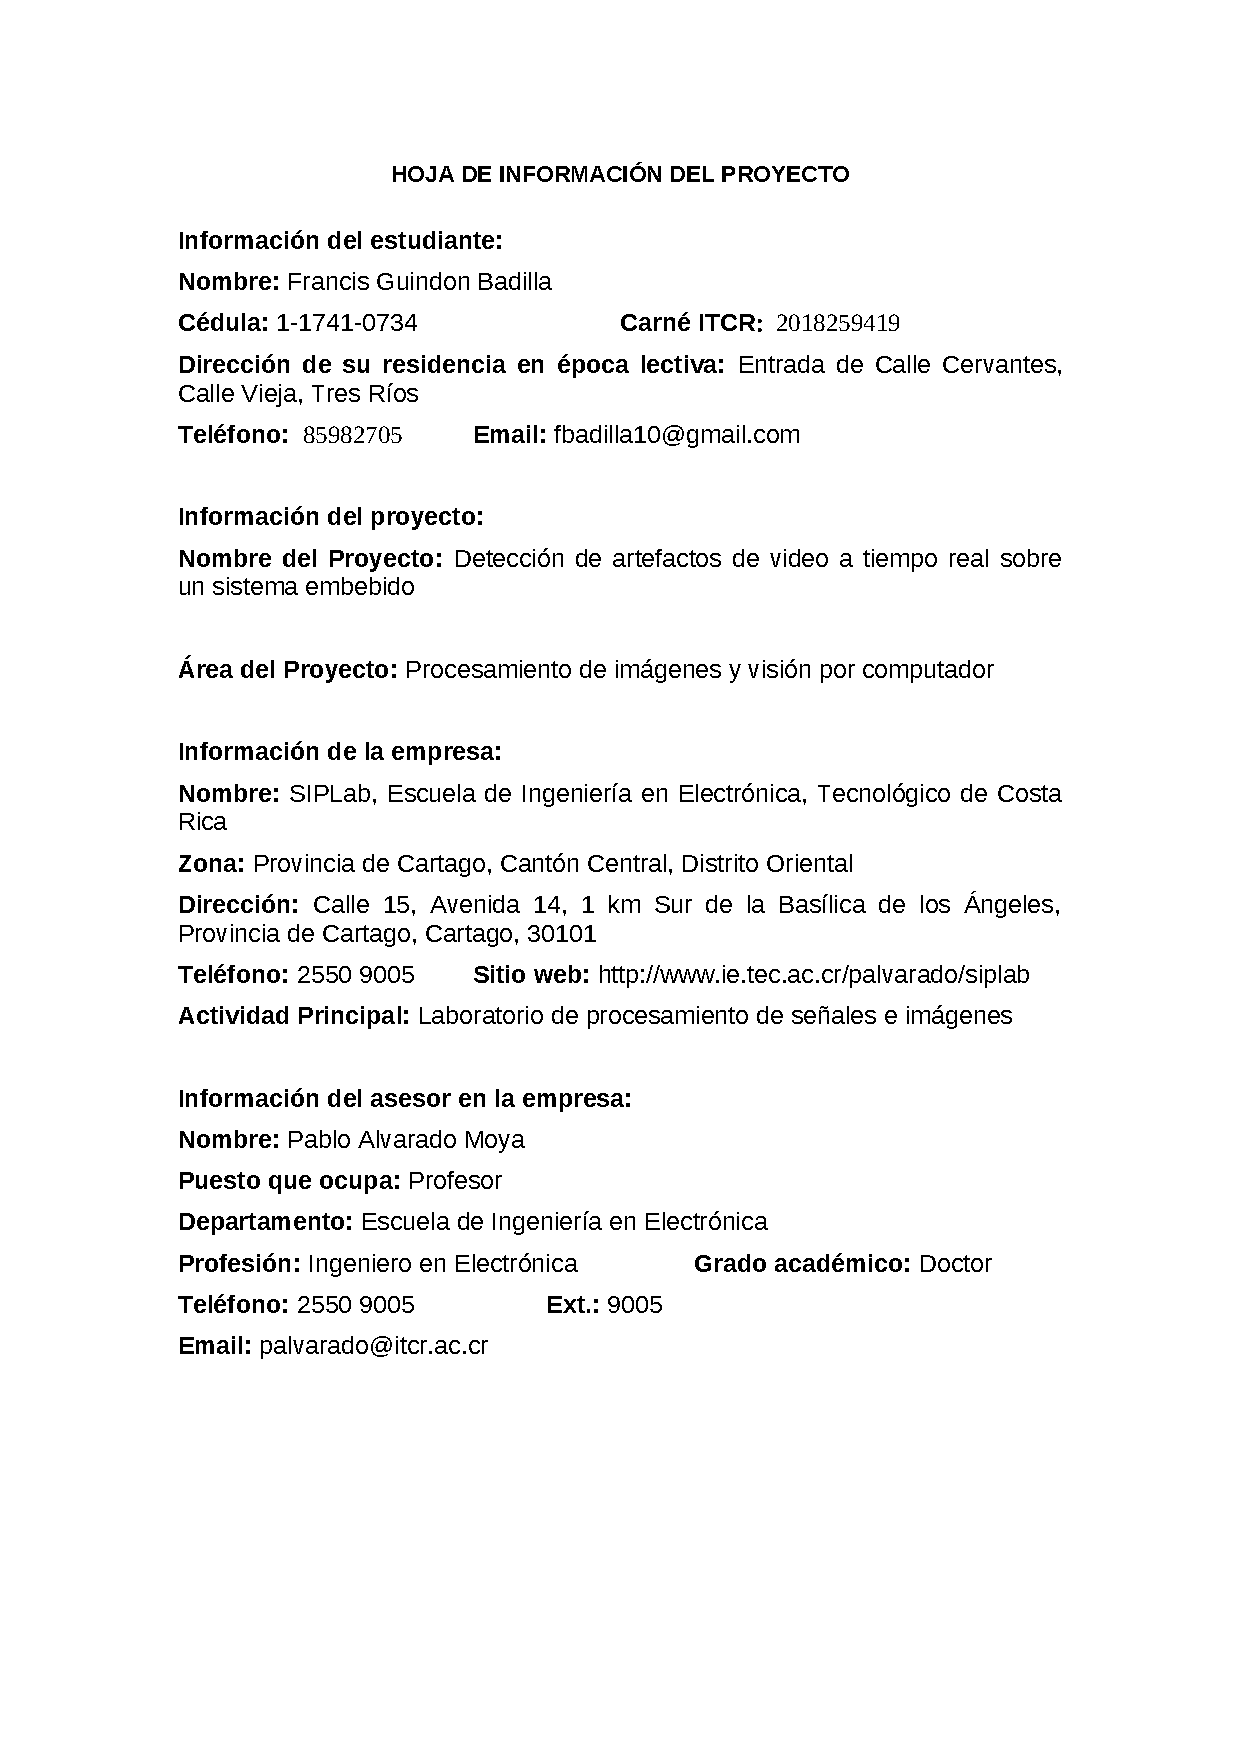
\includepdf[scale=1, offset=3cm -4cm, pagecommand={\textbf{Anexo B}}]{hoja_info.pdf}


  %----------------------------------------------------------------------------
  \backmatter
  %----------------------------------------------------------------------------

  \printindex                % insert index into document. Don't forget to call
                             % "makeindex filename" first.
\end{document}
